\documentclass[12pt,a4paper]{article}

% ── Packages ──────────────────────────────────────────────────────────────────
\usepackage[T1]{fontenc}
\usepackage[utf8]{inputenc}
\usepackage[english]{babel}
\usepackage{lmodern}
\usepackage{microtype}
\usepackage{geometry}
\geometry{left=2.5cm, right=2.5cm, top=2.5cm, bottom=2.5cm}

\usepackage{amsmath, amssymb}
\usepackage{graphicx}
\usepackage{subcaption}
\usepackage{float}
\usepackage{booktabs}
\usepackage{array}
\usepackage{xcolor}
\usepackage{hyperref}
\usepackage{enumitem}
\usepackage{fancyhdr}
\usepackage{titlesec}
\usepackage{caption}
\usepackage{parskip}
\usepackage{titling}

% ── Colors ────────────────────────────────────────────────────────────────────
\definecolor{myblue}{RGB}{30, 90, 160}
\definecolor{mygray}{RGB}{100, 100, 100}
\definecolor{mygreen}{RGB}{0, 120, 60}
\definecolor{myred}{RGB}{180, 30, 30}

% ── Hyperref ──────────────────────────────────────────────────────────────────
\hypersetup{colorlinks=true, linkcolor=myblue, citecolor=myblue, urlcolor=myblue}

% ── Section formatting ────────────────────────────────────────────────────────
\titleformat{\section}{\large\bfseries\color{myblue}}{\thesection}{1em}{}[\titlerule]
\titleformat{\subsection}{\normalsize\bfseries\color{myblue}}{\thesubsection}{1em}{}
\titleformat{\subsubsection}{\normalsize\itshape\color{mygray}}{\thesubsubsection}{1em}{}

% ── Spacing ───────────────────────────────────────────────────────────────────
\titlespacing{\section}{0pt}{8pt}{4pt}
\titlespacing{\subsection}{0pt}{6pt}{2pt}
\setlength{\parskip}{4pt}

% ── Header / footer ───────────────────────────────────────────────────────────
\pagestyle{fancy}
\fancyhf{}
\rhead{\textcolor{mygray}{\small Blind Motion Deblurring for License Plates}}
\lhead{\textcolor{mygray}{\small Computer Vision Report}}
\cfoot{\thepage}

% ── Caption style ─────────────────────────────────────────────────────────────
\captionsetup{font=small, labelfont=bf, labelsep=period, skip=4pt}

% ── Graphics path ─────────────────────────────────────────────────────────────
\graphicspath{{notebook_outputs/}{input/}}

% ── Math operators ────────────────────────────────────────────────────────────
\DeclareMathOperator*{\argmin}{arg\,min}
\newcommand{\norm}[1]{\left\lVert#1\right\rVert}

% ══════════════════════════════════════════════════════════════════════════════
\begin{document}
% ══════════════════════════════════════════════════════════════════════════════

% ── Compact title block ───────────────────────────────────────────────────────
\begin{center}
  {\LARGE\bfseries\color{myblue} Blind Motion Deblurring and OCR for License Plates}\\[0.4em]
  {\large A Classical Image Processing Pipeline Without Deep Learning}\\[0.3em]
  {\small Computer Vision --- 2025/2026 \quad|\quad \today}
\end{center}

\noindent\rule{\linewidth}{0.5pt}

\noindent\textbf{Abstract.}
This report presents a fully classical, training-free pipeline for blind motion deblurring
of license plate images. Given only the blurred observation --- with no sharp reference and
no learned prior --- the system estimates the motion blur kernel (angle and length) from the
image spectrum and cepstrum, constructs a spatially-varying PSF via Thin Plate Spline
interpolation, and recovers the sharp image through Wiener filtering followed by
Half-Quadratic Splitting (HQS) with Total Variation regularization.
Two OCR routes are compared: deblurring then recognizing (\emph{Route~1}) versus recognizing
directly on the blurred image (\emph{Route~2}).
Experiments on 8 real license plate images show Route~1 wins in 2 cases, ties in 3, and
loses in 3, revealing the fragility of classical blind deconvolution under challenging
imaging conditions. No neural networks or learned representations are used at any stage.

\noindent\rule{\linewidth}{0.5pt}

\tableofcontents
\vspace{0.5em}

% ══════════════════════════════════════════════════════════════════════════════
\section{Introduction}
% ══════════════════════════════════════════════════════════════════════════════

License plate recognition is a fundamental task in intelligent transportation systems.
In practice, captured images are frequently degraded by motion blur caused by vehicle
movement or camera shake during exposure. This smears character strokes, reduces contrast,
and causes adjacent characters to merge --- severely impairing automatic text recognition.

For blur lengths beyond 10--15 pixels, direct OCR on the blurred image typically fails even
with aggressive contrast enhancement. The classical remedy is \emph{blind deconvolution}:
estimating the unknown blur kernel from the blurred image itself and then inverting the
blurring operator to recover a sharp estimate. This is an ill-posed problem requiring
carefully designed priors about image content and blur structure.

This work implements and evaluates such a pipeline for license plates.
The blur kernel (angle and length) is estimated from the Fourier spectrum and cepstrum,
a spatially-varying PSF is constructed via Thin Plate Spline (TPS) interpolation,
and the image is deblurred by a two-stage Wiener + HQS solver. Two OCR strategies are
compared empirically on 8 real blurred plates.

\textbf{Key constraint:} No deep learning, neural networks, or learned representation
is used at any stage. All components derive from classical signal processing and optimization.

% ══════════════════════════════════════════════════════════════════════════════
\section{Problem Formulation}
% ══════════════════════════════════════════════════════════════════════════════

Motion blur is modelled as linear convolution with additive noise:
\begin{equation}
  \mathbf{y} = k \ast \mathbf{x} + \mathbf{n}
  \label{eq:degradation}
\end{equation}
where $\mathbf{y}$ is the observed blurred image, $\mathbf{x}$ is the unknown sharp image,
$k$ is the \emph{Point Spread Function} (PSF), and $\mathbf{n}$ is sensor noise.
For motion blur, the PSF is a line kernel parameterised by angle $\theta \in [0°, 180°)$
and length $L \in \mathbb{Z}^+$.
Since neither $\mathbf{x}$ nor $k$ is observed, the problem splits into:
\textbf{(1) PSF estimation} from $\mathbf{y}$ alone, and
\textbf{(2) non-blind deconvolution} given $\hat{k}$:
\begin{equation}
  \hat{\mathbf{x}} = \argmin_{\mathbf{x} \geq 0}
    \underbrace{\tfrac{1}{2}\norm{k \ast \mathbf{x} - \mathbf{y}}^2_2}_{\text{data fidelity}}
    + \underbrace{\lambda\,\mathrm{TV}(\mathbf{x})}_{\text{TV regularization}}
    + \underbrace{\gamma\,H(\mathbf{x})}_{\text{Hough geometry}}
  \label{eq:objective}
\end{equation}

The isotropic Total Variation term $\mathrm{TV}(\mathbf{x}) = \sum_{i,j}\norm{\nabla\mathbf{x}_{i,j}}_2$
promotes piecewise-constant regions --- sharp edges with smooth areas --- which is an appropriate
prior for license plate characters on a uniform background.
The Hough geometry term penalizes gradients aligned with the blur direction:
\begin{equation}
  H(\mathbf{x}) = \sum_{i,j}
    \!\left(1 - \cos^2\!\left(\angle\nabla\mathbf{x}_{i,j} - \theta_{\mathrm{plate}}\right)\right)
    \norm{\nabla\mathbf{x}_{i,j}}_2
\end{equation}
Gradients parallel to the blur direction incur zero penalty (preserved); perpendicular
gradients are suppressed, removing blur-direction streaks while keeping real plate structure.

% ══════════════════════════════════════════════════════════════════════════════
\section{Methodology}
% ══════════════════════════════════════════════════════════════════════════════

The full pipeline is illustrated using \texttt{img1.png}
($\mathrm{GT} = \mathtt{GJW115A1138}$, angle $48°$, length $14\,\mathrm{px}$)
as the walkthrough example.

\subsection{Step 1A — Blur Angle Estimation via Hough on FFT}

The Fourier Transform of a motion-blurred image shows a bright stripe along the blur axis
in the log-magnitude spectrum, because the kernel suppresses energy perpendicular to the
motion direction. We exploit this through the \emph{cepstrum}:
\begin{equation}
  C(\mathbf{y}) = \mathcal{F}^{-1}\!\left\{\log\left|\mathcal{F}\{\mathbf{y}\}\right|\right\}
\end{equation}
A Hanning window is applied before the FFT to suppress spectral leakage.
We then scan 360 radial lines through the cepstrum center. For each angle $\alpha$,
we compute the minimum of the Gaussian-smoothed ($\sigma{=}1.5$) radial profile $C_\alpha(r)$.
The angle with the deepest minimum is selected:
$\hat{\theta} = \argmin_{\alpha} \min_{r} C_\alpha(r)$.

\begin{figure}[H]
  \centering
  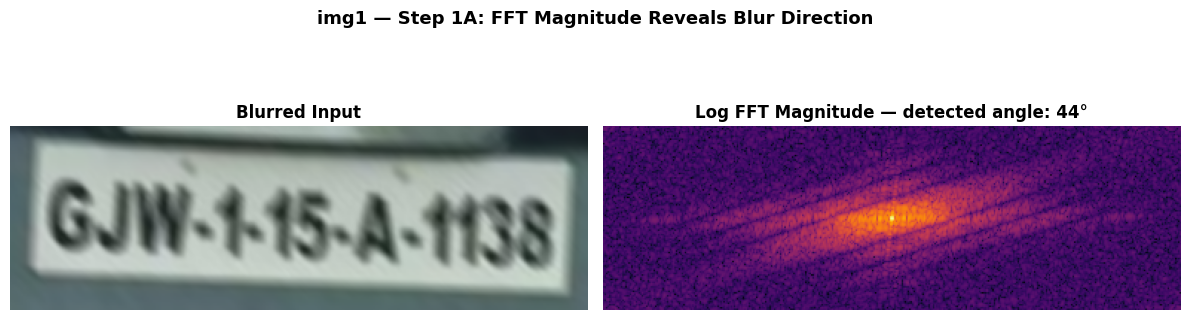
\includegraphics[width=0.95\linewidth]{img1_01_hough_fft.png}
  \caption{\textbf{Step 1A --- FFT Magnitude and Angle Detection (img1).}
    \emph{Left:} Blurred input. \emph{Right:} Log-FFT magnitude (inferno colormap).
    The directional stripe in the spectrum reveals the blur axis;
    the Hough-cepstrum scan detects $48°$.}
  \label{fig:hough_fft}
\end{figure}

\subsection{Step 1B — Blur Length Estimation via Cepstrum}

A motion blur kernel of length $L$ introduces frequency-domain zeros spaced at $1/L$
along the blur axis. In the cepstrum, this periodicity appears as a sharp dip at
distance $L$ from the center. We slice the cepstrum along $\hat{\theta}$ using bilinear
interpolation and locate the minimum:
$\hat{L} = \argmin_{r \in [6,\,\min(H,W)/2-2]} \widetilde{C}_{\hat{\theta}}(r)$,
where $\widetilde{C}$ is the Gaussian-smoothed profile.

\begin{figure}[H]
  \centering
  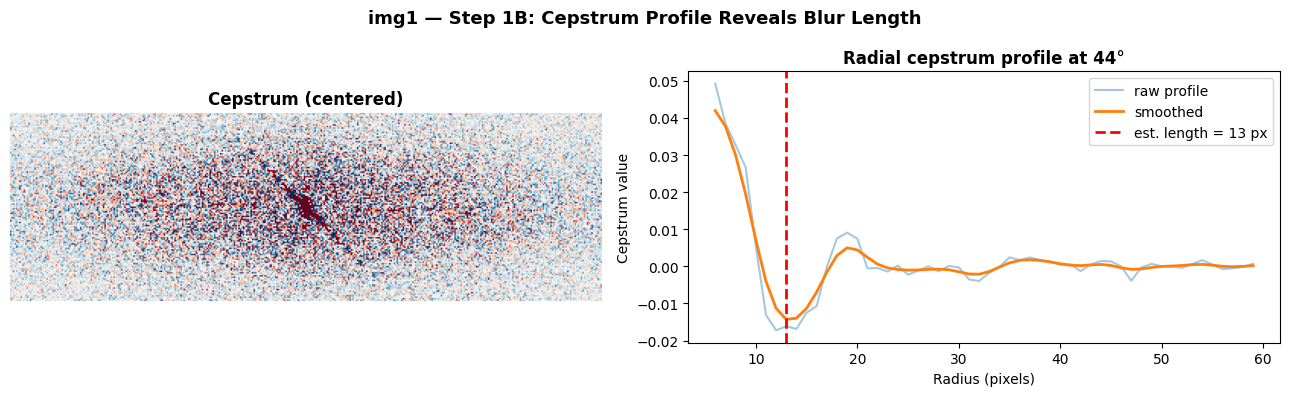
\includegraphics[width=0.95\linewidth]{img1_02_cepstrum.png}
  \caption{\textbf{Step 1B --- Cepstrum Analysis (img1).}
    \emph{Left:} Centered cepstrum.
    \emph{Right:} Radial profile at $48°$; the smoothed curve (solid) reaches its minimum
    at $14\,\mathrm{px}$ (red dashed line) --- the estimated blur length.}
  \label{fig:cepstrum}
\end{figure}

\subsection{Step 1C — Spatially-Varying PSF via Thin Plate Spline}

Camera shake can have rotational components, causing blur to vary spatially across the
image. To capture this, we sample \textbf{9 patches} in a $3{\times}3$ grid and run
Hough+Cepstrum independently on each, obtaining local estimates $(\alpha_i, L_i)$.
Outlier patches (local angle deviating more than $30°$ from the global estimate) are
rejected. A Thin Plate Spline is then fitted through the accepted control points:
\begin{equation}
  f_\mathrm{TPS}(\mathbf{p}) = a_0 + \mathbf{a}^\top\!\mathbf{p}
    + \sum_{i=1}^{N} w_i\,\phi\!\left(\norm{\mathbf{p}-\mathbf{p}_i}_2\right),
  \quad \phi(r)=r^2\log r
  \label{eq:tps}
\end{equation}
producing dense angle and length maps. The center-pixel values give the refined global
estimates; a weighted blend is used:
$L_{\mathrm{final}} = 0.6\,\hat{L}_{\mathrm{cep}} + 0.4\,\hat{L}_{\mathrm{TPS}}$.

\begin{figure}[H]
  \centering
  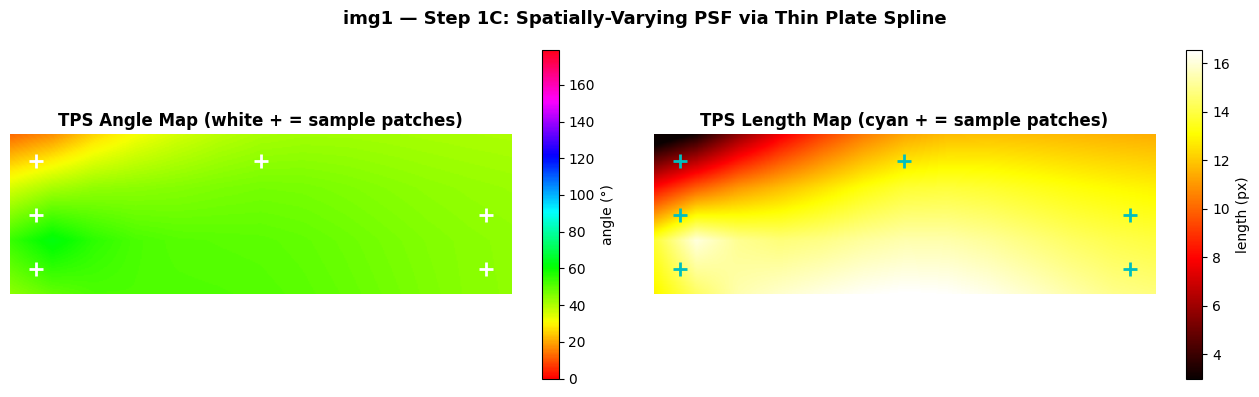
\includegraphics[width=0.95\linewidth]{img1_03_tps_maps.png}
  \caption{\textbf{Step 1C --- Spatially-Varying PSF Maps via TPS (img1).}
    \emph{Left:} Angle map (HSV colormap); white crosses mark sample patches.
    \emph{Right:} Length map (hot colormap); cyan crosses mark sample locations.
    The smooth spatial variation validates the near-uniform blur assumption for img1.}
  \label{fig:tps_maps}
\end{figure}

\subsection{Step 1D — Motion Blur Kernel Construction}

Given $(\hat{\theta}, \hat{L})$, the kernel is built using bilinear splatting for
sub-pixel accuracy --- each point along the motion trajectory distributes its weight
to the four nearest integer pixels, avoiding aliasing from nearest-neighbor rounding.
The kernel is normalized to sum to 1.
Figure~\ref{fig:kernels} shows the estimated kernels for the three images analysed in detail.

\begin{figure}[H]
  \centering
  \begin{subfigure}[b]{0.3\linewidth}
    \centering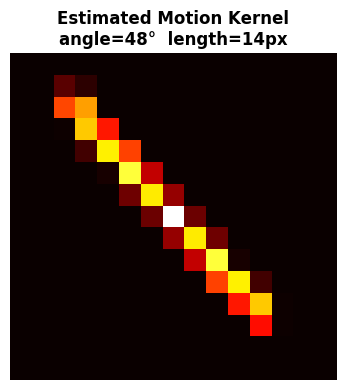
\includegraphics[width=\linewidth]{img1_04_kernel.png}
    \caption{img1: $48°$, $14\,\mathrm{px}$}
  \end{subfigure}\hfill
  \begin{subfigure}[b]{0.3\linewidth}
    \centering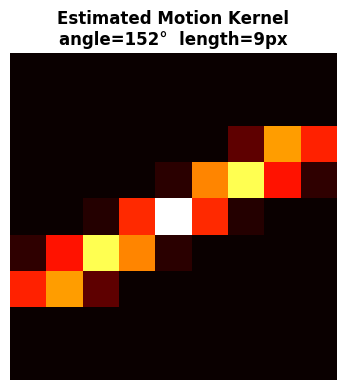
\includegraphics[width=\linewidth]{img5_04_kernel.png}
    \caption{img5: $152°$, $9\,\mathrm{px}$}
  \end{subfigure}\hfill
  \begin{subfigure}[b]{0.3\linewidth}
    \centering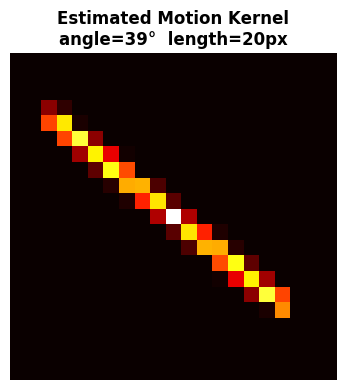
\includegraphics[width=\linewidth]{img8_04_kernel.png}
    \caption{img8: $39°$, $20\,\mathrm{px}$}
  \end{subfigure}
  \caption{\textbf{Step 1D --- Estimated Motion Blur Kernels} (hot colormap).
    img1: clean diagonal line at $48°$.
    img8: longest kernel in the dataset ($20\,\mathrm{px}$).
    img5: near-horizontal at $152°$ --- this direction will prove problematic for deconvolution.}
  \label{fig:kernels}
\end{figure}

\subsection{Step 2 — Wiener Rough Pass and Character Mask}

The Wiener filter solves the deconvolution in the Fourier domain:
\begin{equation}
  \hat{X}(\omega) = \frac{\overline{K}(\omega)}{|K(\omega)|^2 + K_{\mathrm{noise}}} \cdot Y(\omega)
  \label{eq:wiener}
\end{equation}
$K_{\mathrm{noise}}$ is estimated adaptively via the Median Absolute Deviation (MAD)
on the residual between the image and its Gaussian-smoothed version:
$\hat{\sigma}_n = \mathrm{median}|\mathbf{y} - G_{\sigma=1}\ast\mathbf{y}|\,/\,0.6745$,
then $K_{\mathrm{noise}} = \mathrm{clip}(\hat{\sigma}_n^2/\mathrm{Var}(\mathbf{y}),\;10^{-4},\;0.1)$.
Filtering is applied per RGB channel. The output is a rough deblurred image --- fast but
subject to ringing artifacts near kernel zeros. A binary character mask is extracted from
the Wiener output via Otsu thresholding (maximizing between-class variance) to localize
plate characters for the subsequent HQS solver.

\begin{figure}[H]
  \centering
  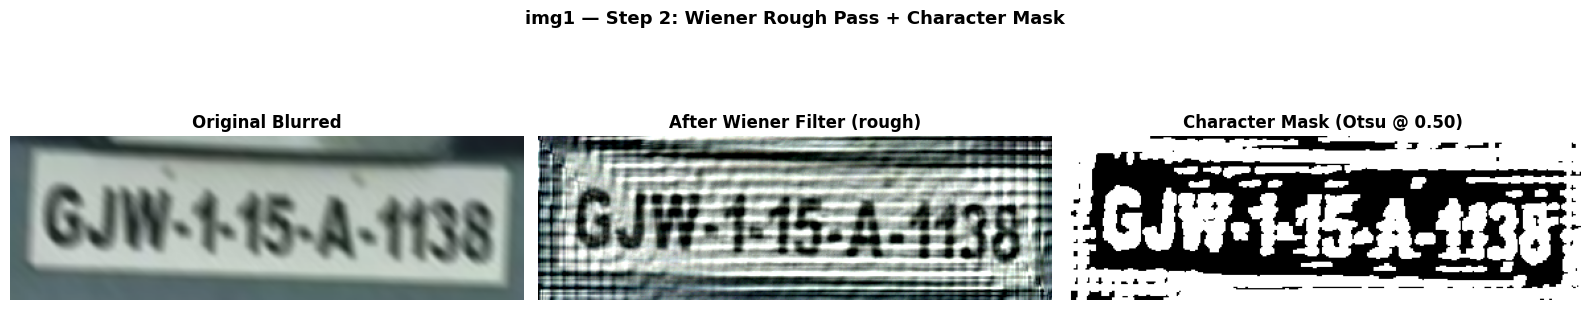
\includegraphics[width=0.95\linewidth]{img1_05_wiener_mask.png}
  \caption{\textbf{Step 2 --- Wiener Rough Pass and Character Mask (img1).}
    \emph{Left:} Original blurred image.
    \emph{Center:} Wiener output --- characters recovered but ringing visible near edges.
    \emph{Right:} Otsu binary mask correctly localizing character regions.}
  \label{fig:wiener_mask}
\end{figure}

\subsection{Step 3 — Fine Deblurring: Half-Quadratic Splitting (HQS)}

Solving objective~\eqref{eq:objective} jointly is expensive because the data fidelity
couples all pixels through convolution. HQS introduces auxiliary variable $\mathbf{z}$
to decouple the problem:
\begin{equation}
  \min_{\mathbf{x},\mathbf{z}}\;
  \tfrac{1}{2}\norm{k\ast\mathbf{x}-\mathbf{y}}^2_2
  + \tfrac{\mu}{2}\norm{\mathbf{x}-\mathbf{z}}^2_2
  + \lambda\,\mathrm{TV}(\mathbf{z}) + \gamma\,H(\mathbf{z})
\end{equation}
This alternates between:
\textbf{x-step} --- closed-form Wiener in the Fourier domain (deconvolution only):
$\mathbf{x}^{(t+1)} = \mathcal{F}^{-1}\!\left\{(\overline{K}\cdot\mathcal{F}\{\mathbf{y}\} + \mu\mathcal{F}\{\mathbf{z}^{(t)}\})/(|K|^2+\mu)\right\}$;
and \textbf{z-step} --- proximal TV+Hough minimization via Chambolle--Pock (denoising only, no convolution).
The outer loop runs 8 iterations; each z-step runs 40 Chambolle--Pock iterations.
$\mu$ increases progressively so $\mathbf{x}$ and $\mathbf{z}$ converge to the same solution.
After the HQS loop, directional unsharp masking (perpendicular to blur) sharpens
cross-blur edges, and cross-channel luminance coupling suppresses color fringing.

% ══════════════════════════════════════════════════════════════════════════════
\section{Experimental Pipeline}
% ══════════════════════════════════════════════════════════════════════════════

\subsection{Dataset and Setup}

The dataset consists of 8 real-world blurred license plate images (\texttt{img1}--\texttt{img8}),
all genuine captures with no artificially synthesized blur. Ground truth plate strings are
known for all 8 (see Table~\ref{tab:results}). No training data or reference sharp images
are used at any stage.

\begin{table}[H]
  \centering
  \caption{Pipeline stages, methods, and outputs.}
  \label{tab:pipeline}
  \small
  \begin{tabular}{@{}lll@{}}
    \toprule
    \textbf{Stage} & \textbf{Method} & \textbf{Output} \\
    \midrule
    Angle estimation    & Hough scan on cepstrum of FFT (360 angles)       & $\hat{\theta}$ (degrees) \\
    Length estimation   & Radial cepstrum profile minimum                  & $\hat{L}$ (pixels) \\
    Spatial variation   & TPS on 9 local patch estimates                   & Per-pixel angle/length maps \\
    Kernel construction & Bilinear-splatted normalized line kernel          & $\hat{k}$ ($p{\times}p$) \\
    Rough deblur        & Wiener filter (MAD-adaptive $K_{\mathrm{noise}}$) & Rough RGB + character mask \\
    Fine deblur         & HQS: 8 outer $\times$ 40 TV-prox iterations      & Final sharp RGB image \\
    OCR Route 1         & \texttt{recognize(deblurred\_image)}             & Plate text from deblurred \\
    OCR Route 2         & \texttt{recognize(blurred\_image)}               & Plate text from blurred \\
    \bottomrule
  \end{tabular}
\end{table}

\subsection{OCR Module}

The OCR module (\texttt{ocr\_plate.py}) is a fully standalone classical recognizer with
zero knowledge of deblurring. Its preprocessing --- plate crop, inner crop, CLAHE,
NLM denoising, Gaussian+Otsu binarization, morphological cleaning --- serves binarization
quality only, not motion-blur recovery. Tesseract is called with 80 strategy combinations
(8 preprocessing variants $\times$ 5 PSM modes $\times$ 2 OEM settings); a classical
fallback using HOG+NCC and Hu moments is used when Tesseract returns no valid result.
\textbf{The two routes differ only in what image is passed to this module}: the HQS
output (Route~1) or the original blurred image (Route~2).

\subsection{Evaluation Metric}

Character-level positional accuracy against the ground truth string $s^*$:
\begin{equation}
  \mathrm{Acc}(\hat{s}, s^*) = \frac{1}{|s^*|} \sum_{i=1}^{\min(|\hat{s}|,|s^*|)} \mathbf{1}[\hat{s}_i = s^*_i]
\end{equation}
This penalizes both character substitutions and length mismatches.

% ══════════════════════════════════════════════════════════════════════════════
\section{Results}
% ══════════════════════════════════════════════════════════════════════════════

Figure~\ref{fig:img1_4panel} shows the complete pipeline output for \texttt{img1}
(favorable case: large blur, good contrast, reliable kernel estimate).
Figure~\ref{fig:all_4panel} summarizes all 8 plates side-by-side.

\begin{figure}[H]
  \centering
  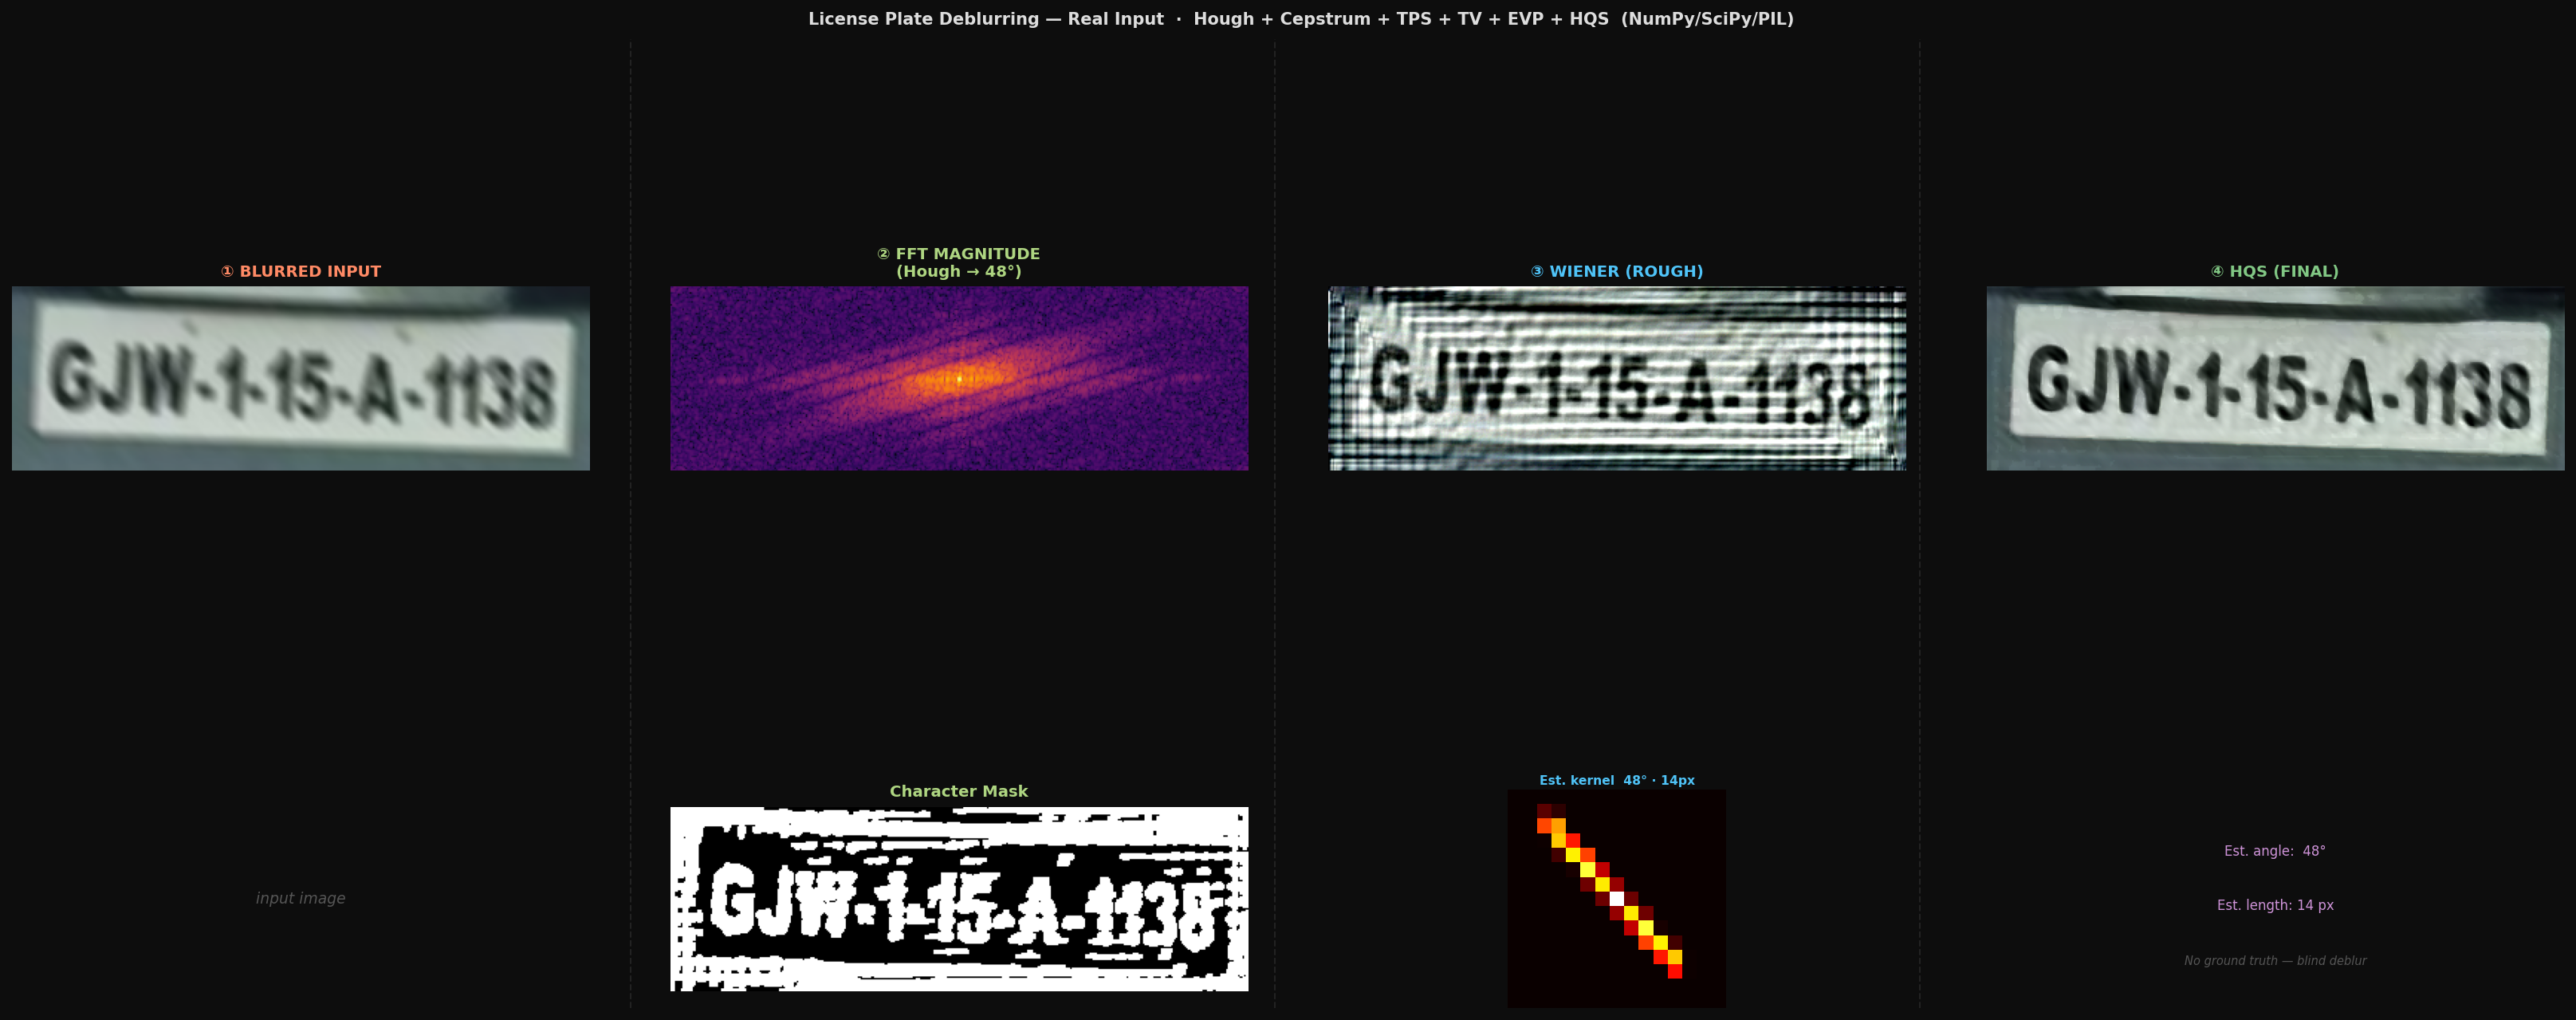
\includegraphics[width=\linewidth]{img1_07_4panel_figure.png}
  \caption{\textbf{Full pipeline output for img1}
    ($\mathrm{GT}{=}\mathtt{GJW115A1138}$, $48°$, $14\,\mathrm{px}$).
    Panel 1: blurred input. Panel 2: log-FFT magnitude.
    Panel 3: Wiener rough pass. Panel 4: final HQS output.
    Route~1 OCR: \texttt{GJW615A1138} (9/11 correct).}
  \label{fig:img1_4panel}
\end{figure}

\begin{figure}[H]
  \centering
  \begin{subfigure}[b]{0.49\linewidth}
    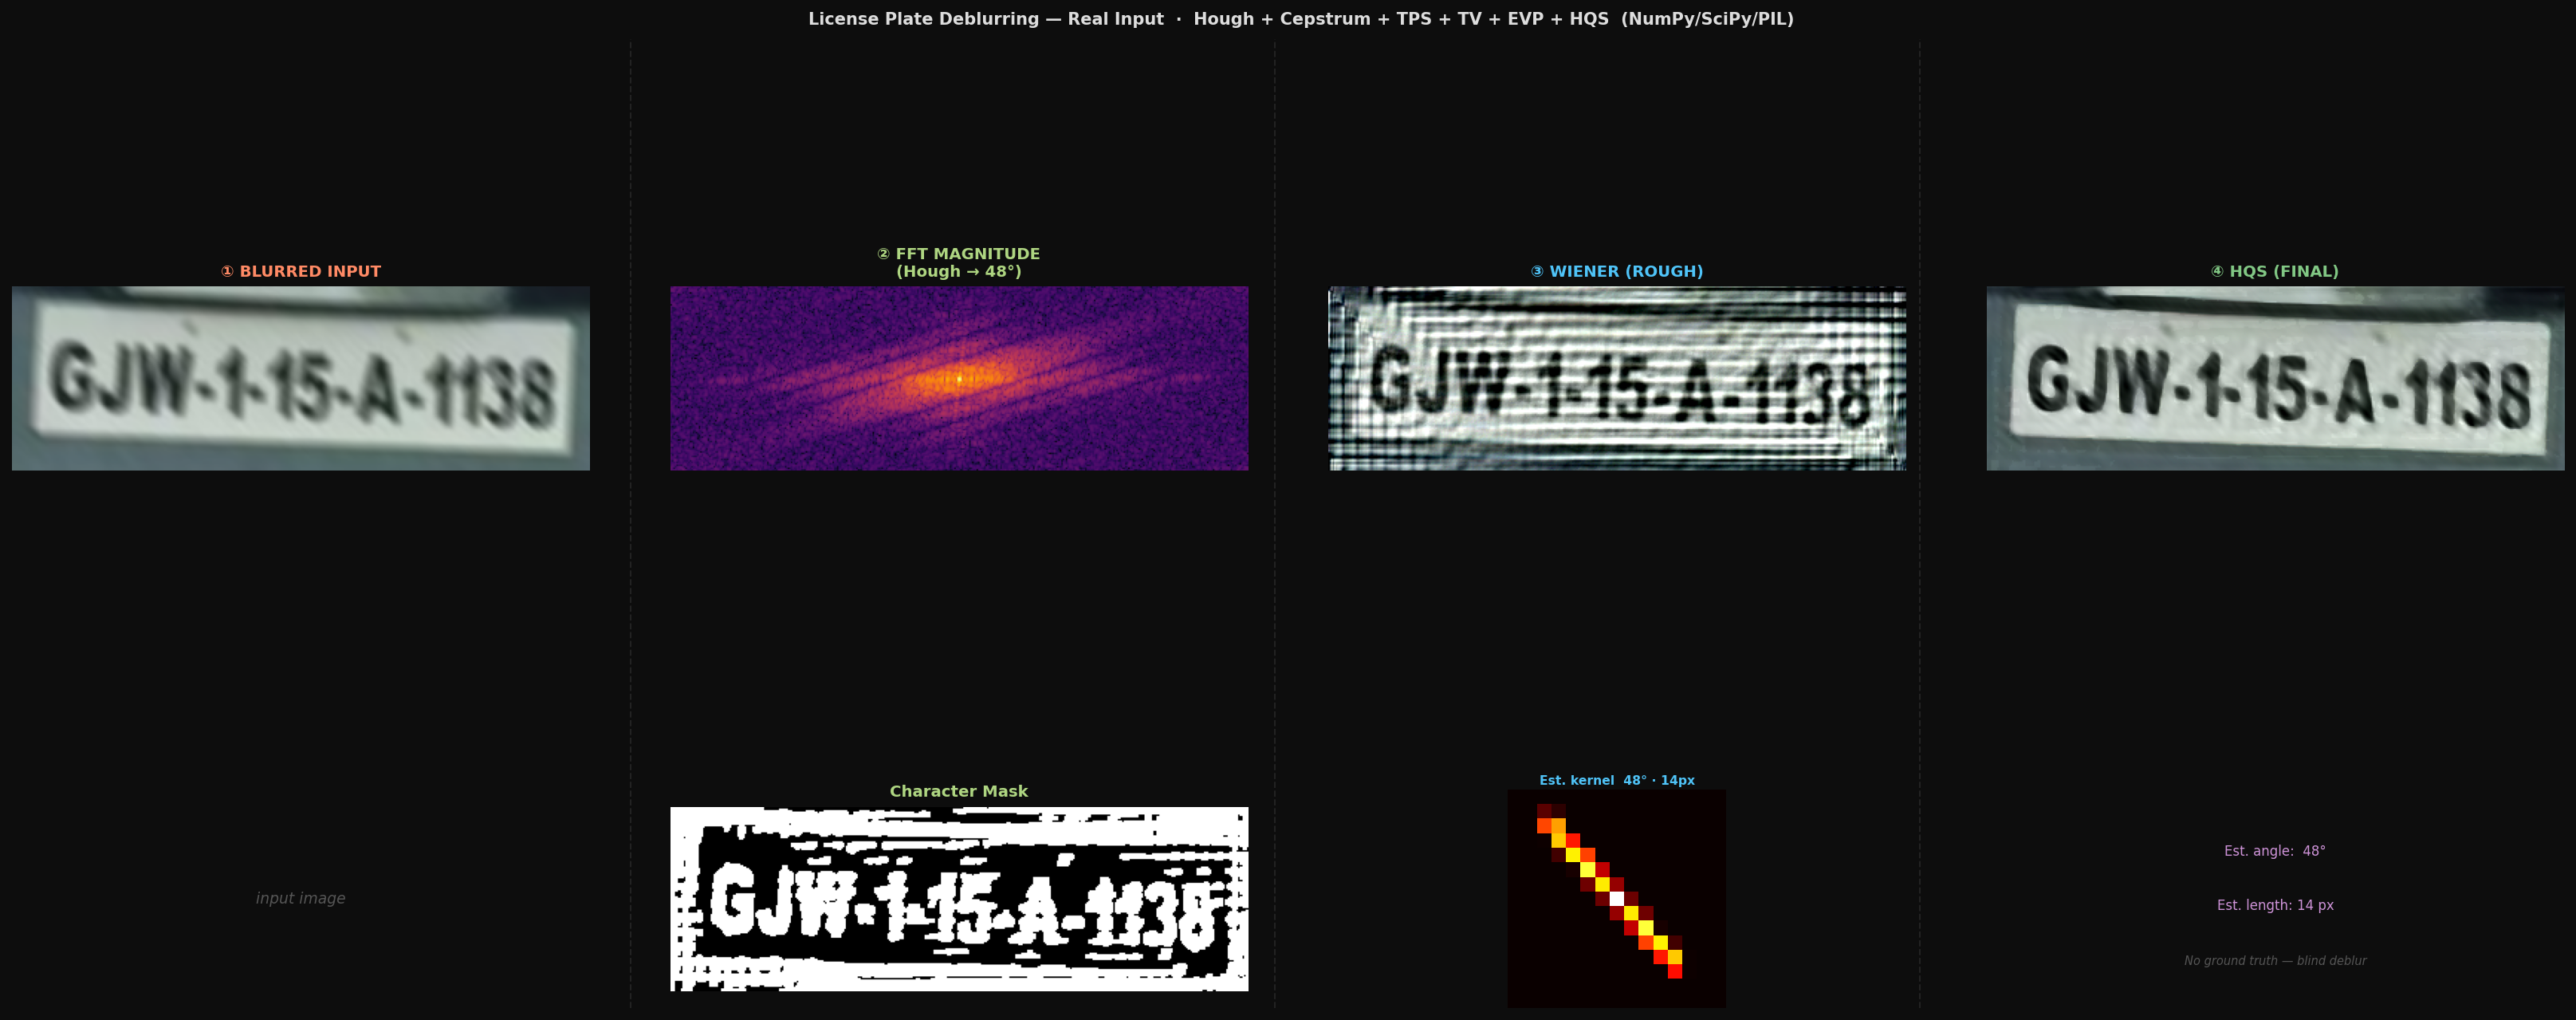
\includegraphics[width=\linewidth]{img1_07_4panel_figure.png}
    \caption{img1: \texttt{GJW115A1138}, $48°$, $14\,\mathrm{px}$}
  \end{subfigure}\hfill
  \begin{subfigure}[b]{0.49\linewidth}
    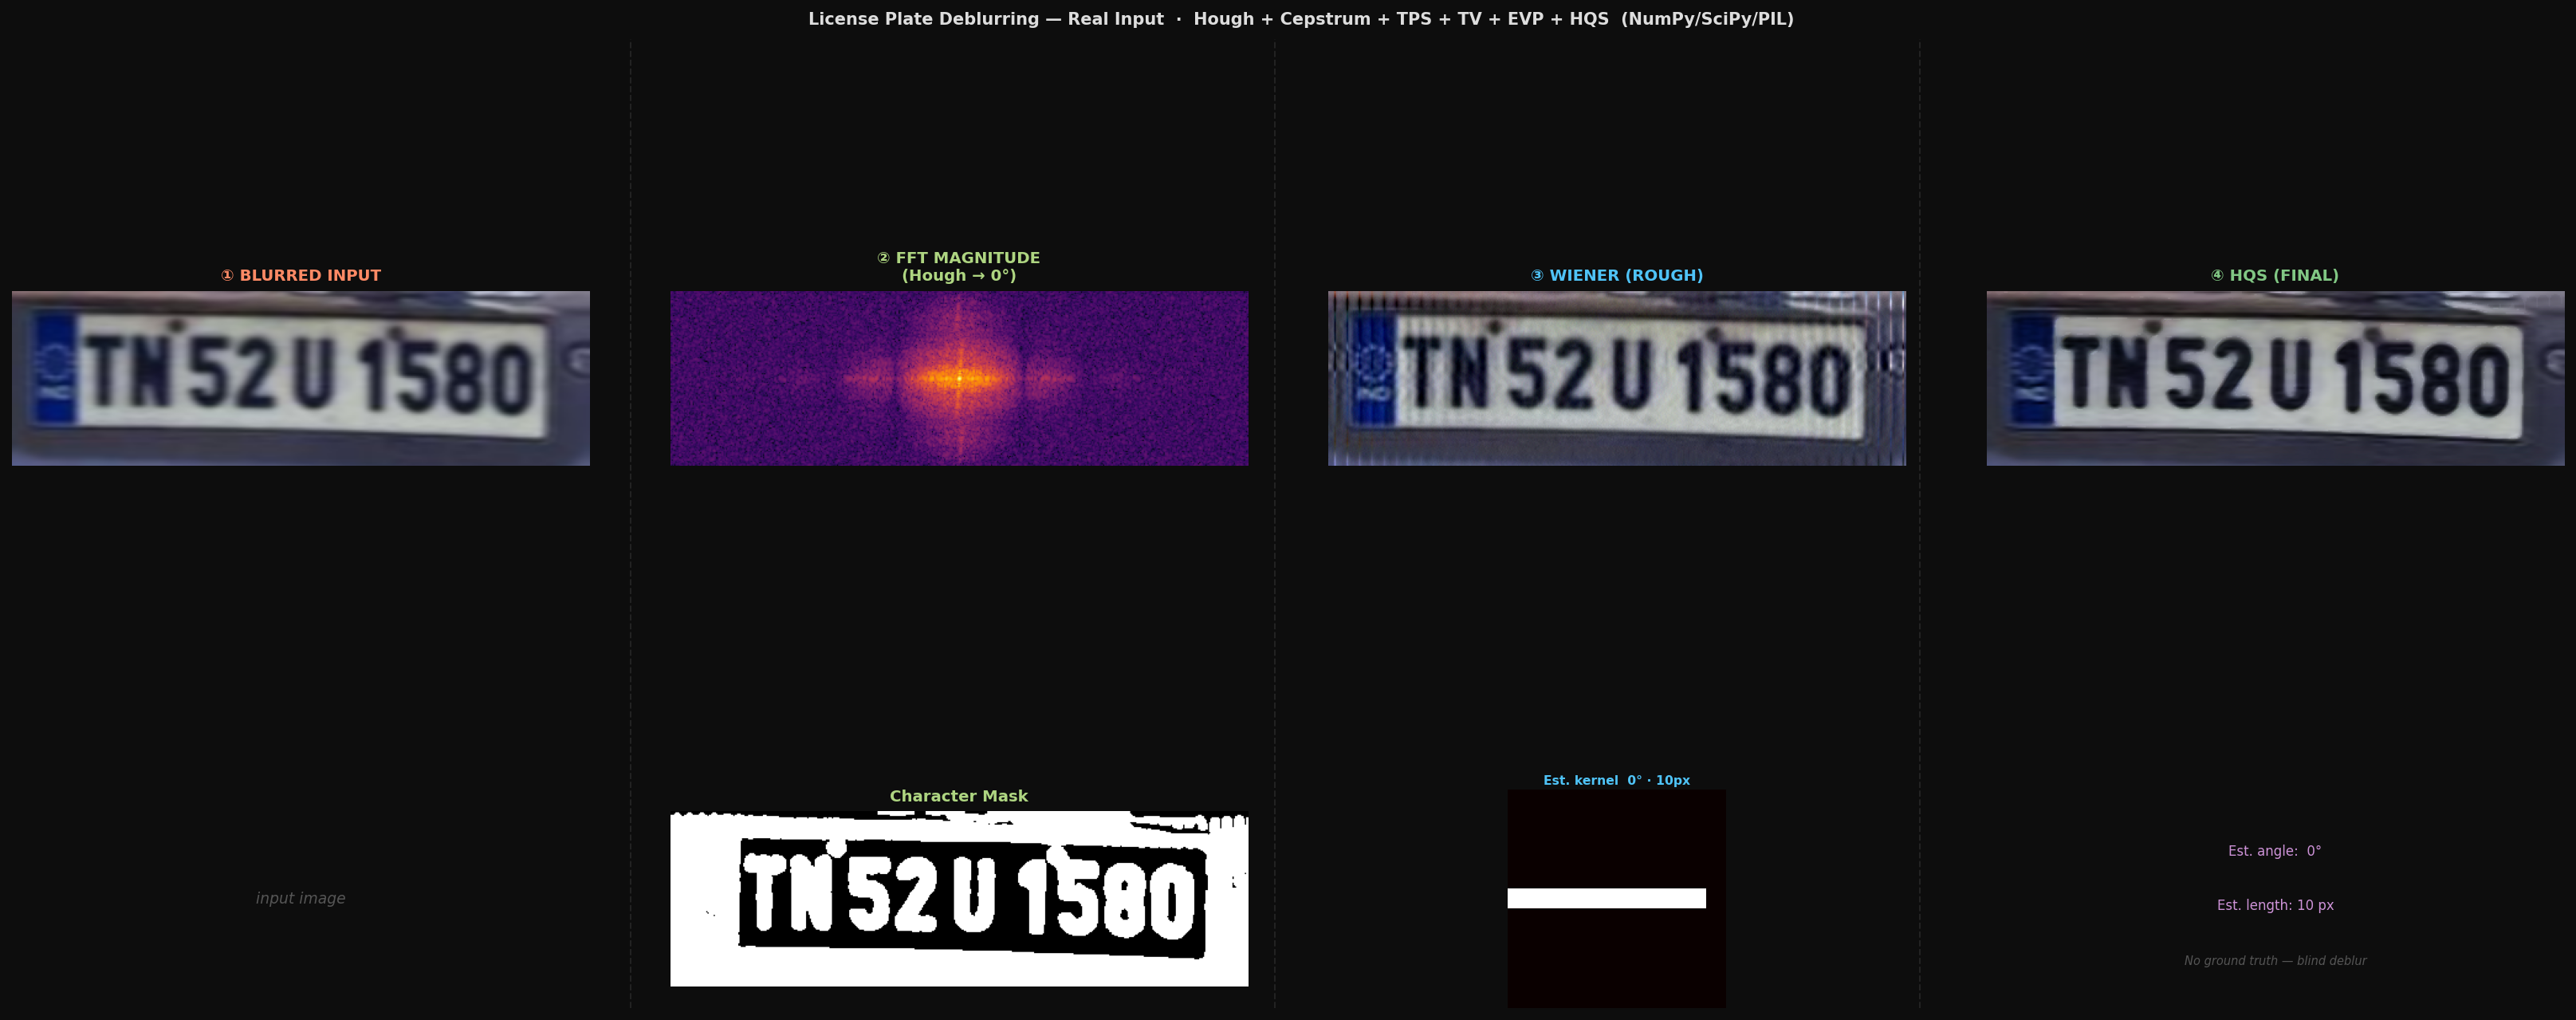
\includegraphics[width=\linewidth]{img2_07_4panel_figure.png}
    \caption{img2: \texttt{TN52U1580}, $0°$, $10\,\mathrm{px}$}
  \end{subfigure}\vspace{0.3em}
  \begin{subfigure}[b]{0.49\linewidth}
    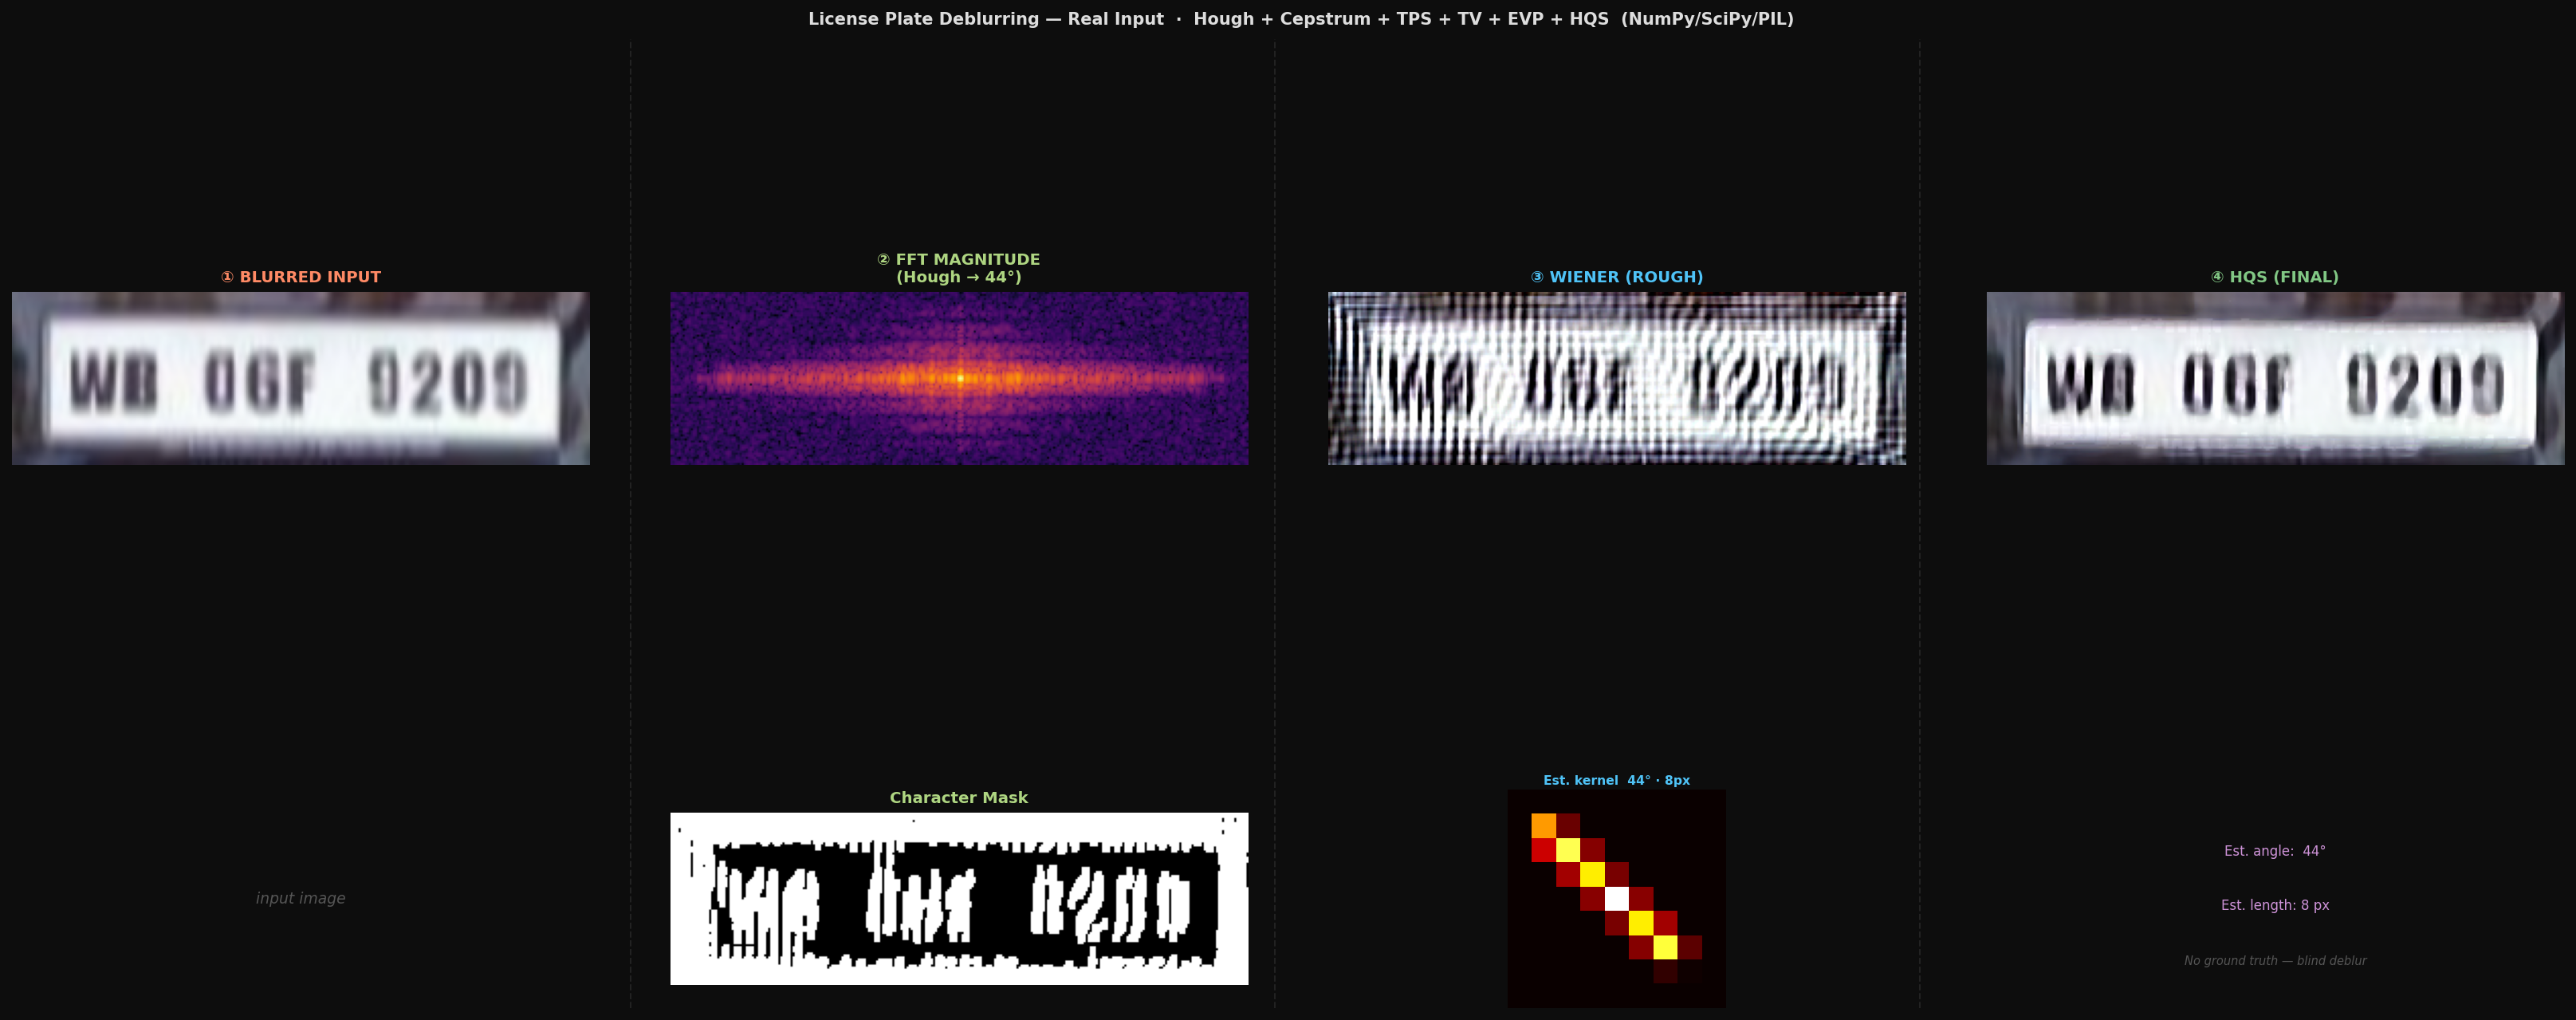
\includegraphics[width=\linewidth]{img3_07_4panel_figure.png}
    \caption{img3: \texttt{WB06F9209}, $44°$, $8\,\mathrm{px}$}
  \end{subfigure}\hfill
  \begin{subfigure}[b]{0.49\linewidth}
    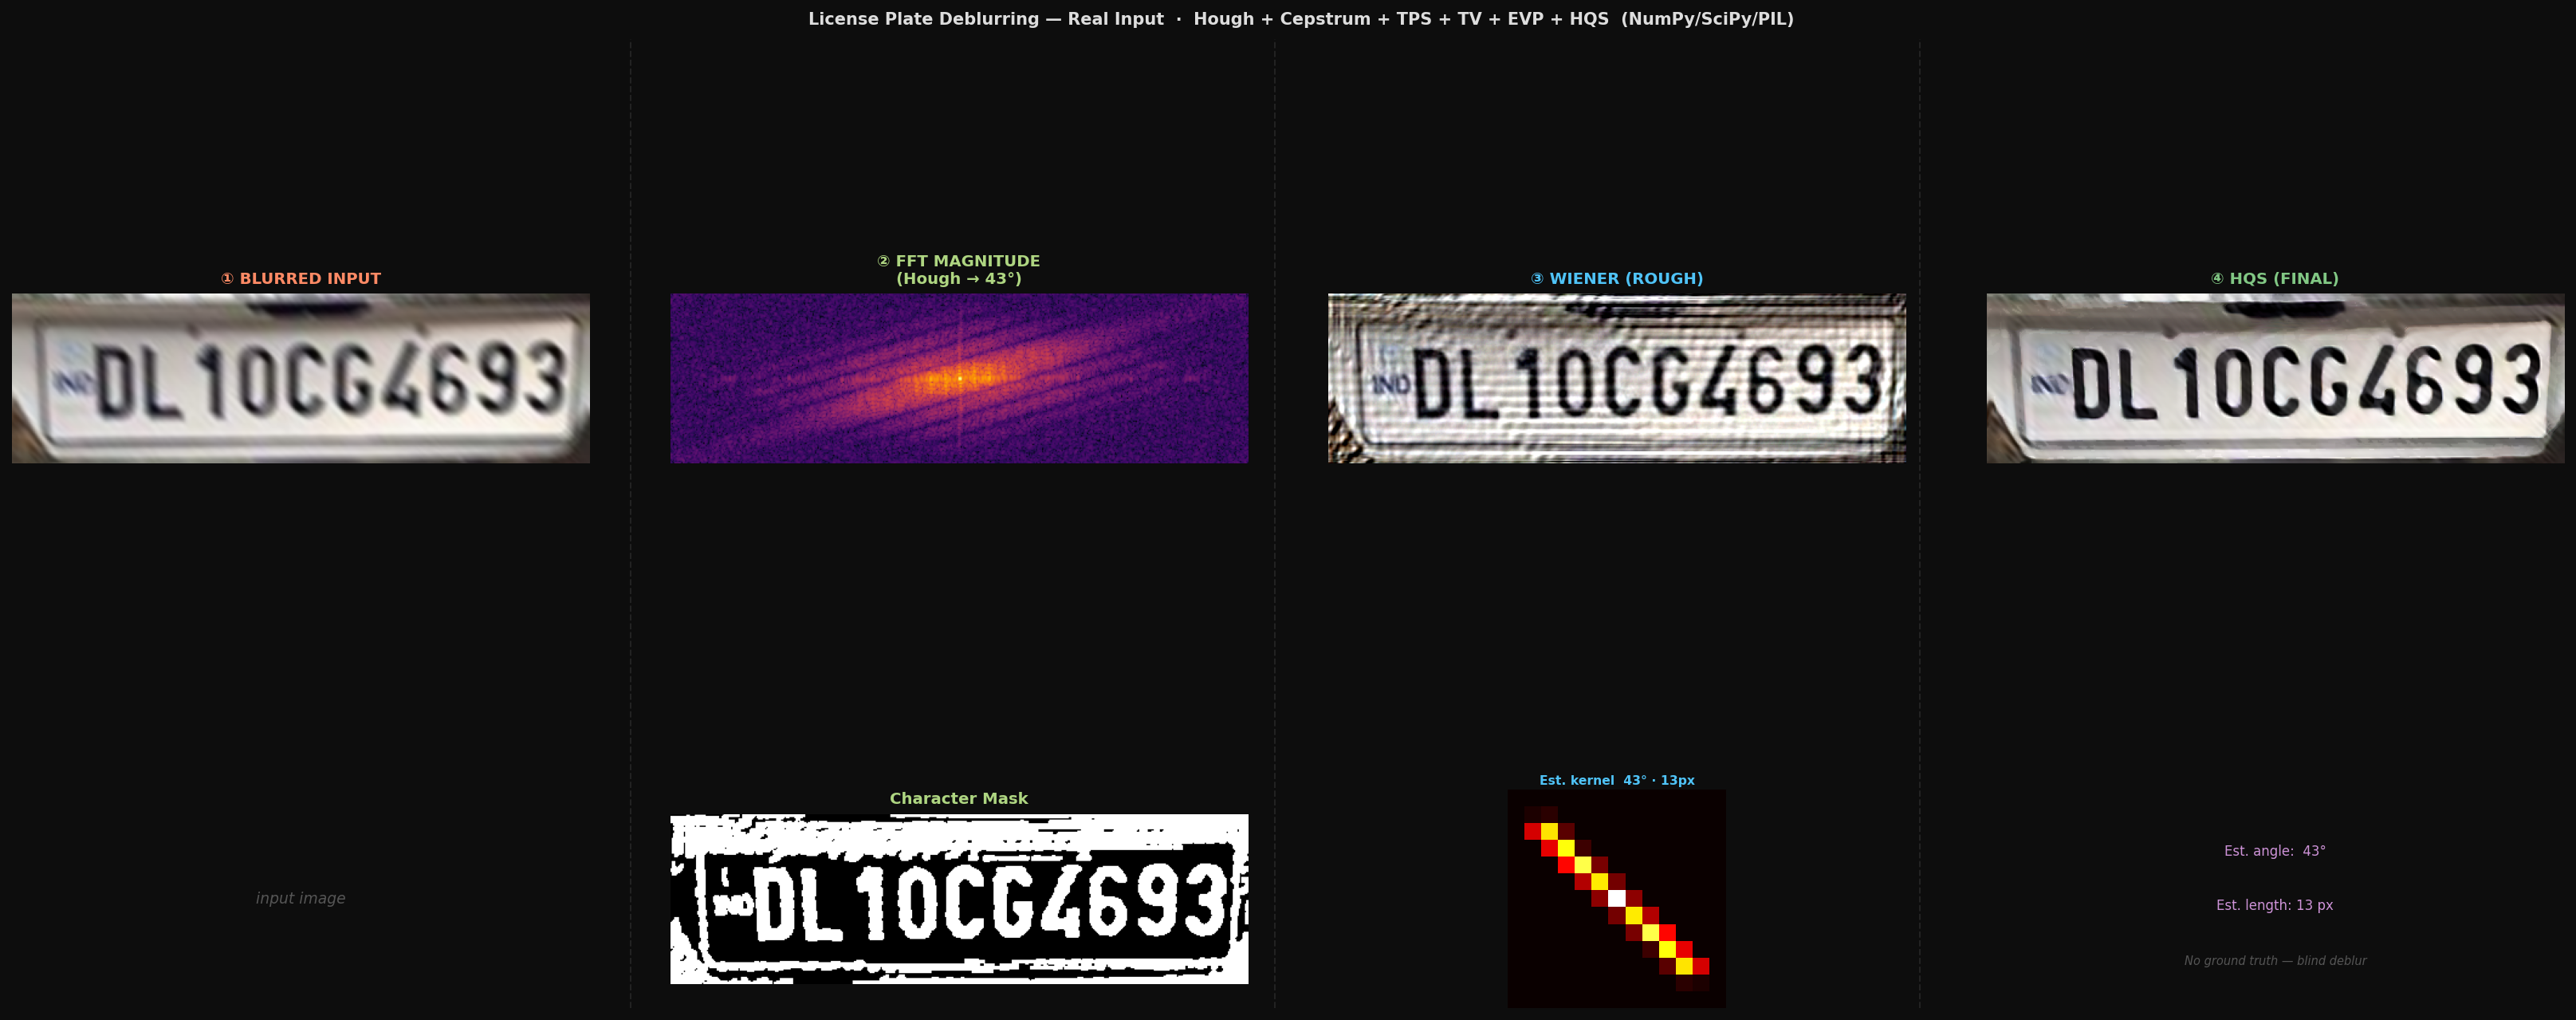
\includegraphics[width=\linewidth]{img4_07_4panel_figure.png}
    \caption{img4: \texttt{DL10CG4693}, $43°$, $13\,\mathrm{px}$}
  \end{subfigure}\vspace{0.3em}
  \begin{subfigure}[b]{0.49\linewidth}
    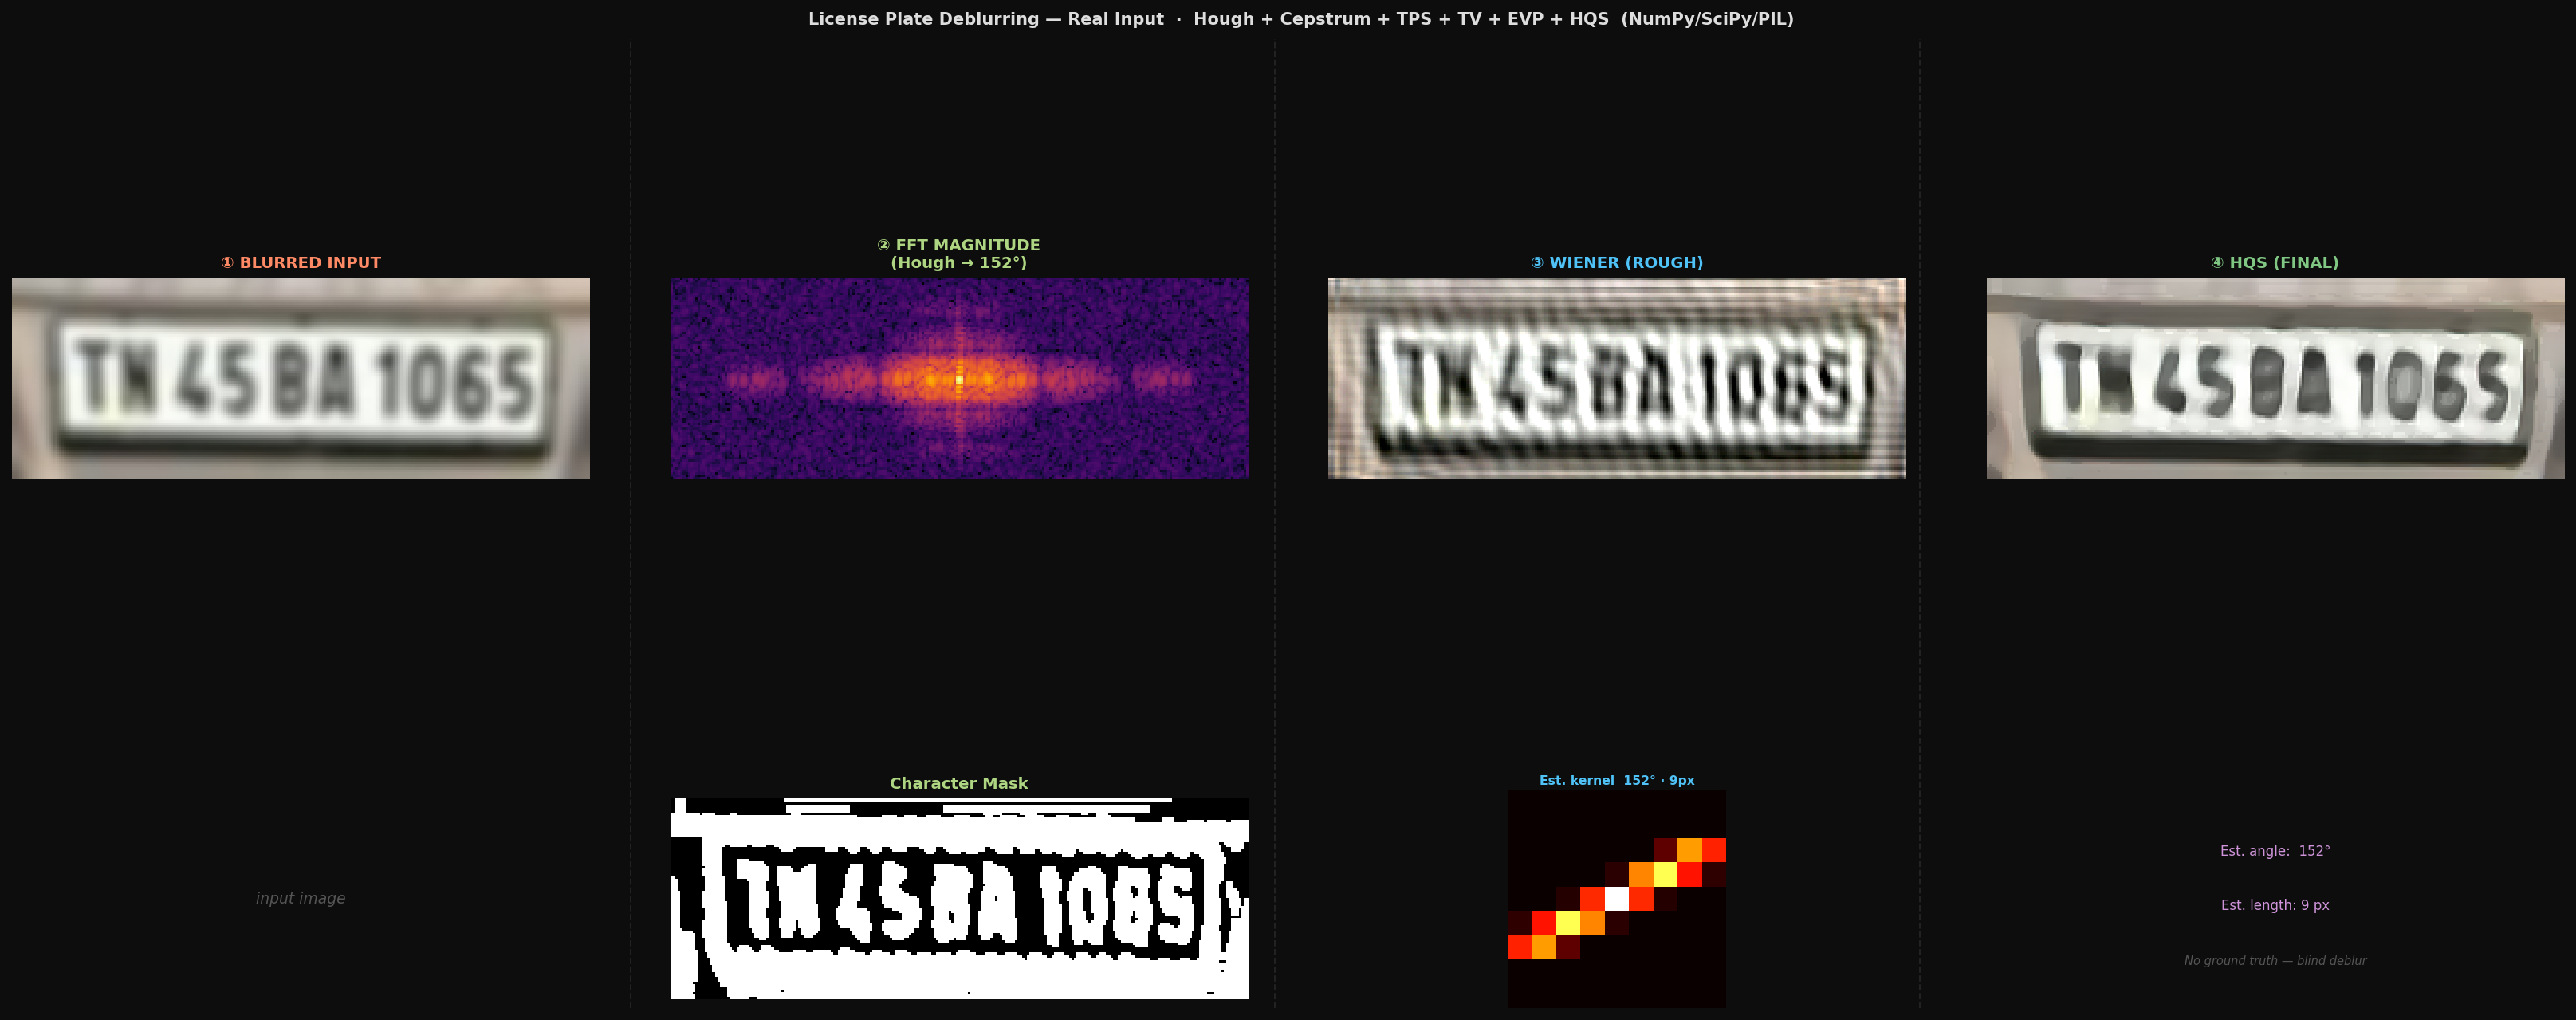
\includegraphics[width=\linewidth]{img5_07_4panel_figure.png}
    \caption{img5: \texttt{TN45BA1065}, $152°$, $9\,\mathrm{px}$}
  \end{subfigure}\hfill
  \begin{subfigure}[b]{0.49\linewidth}
    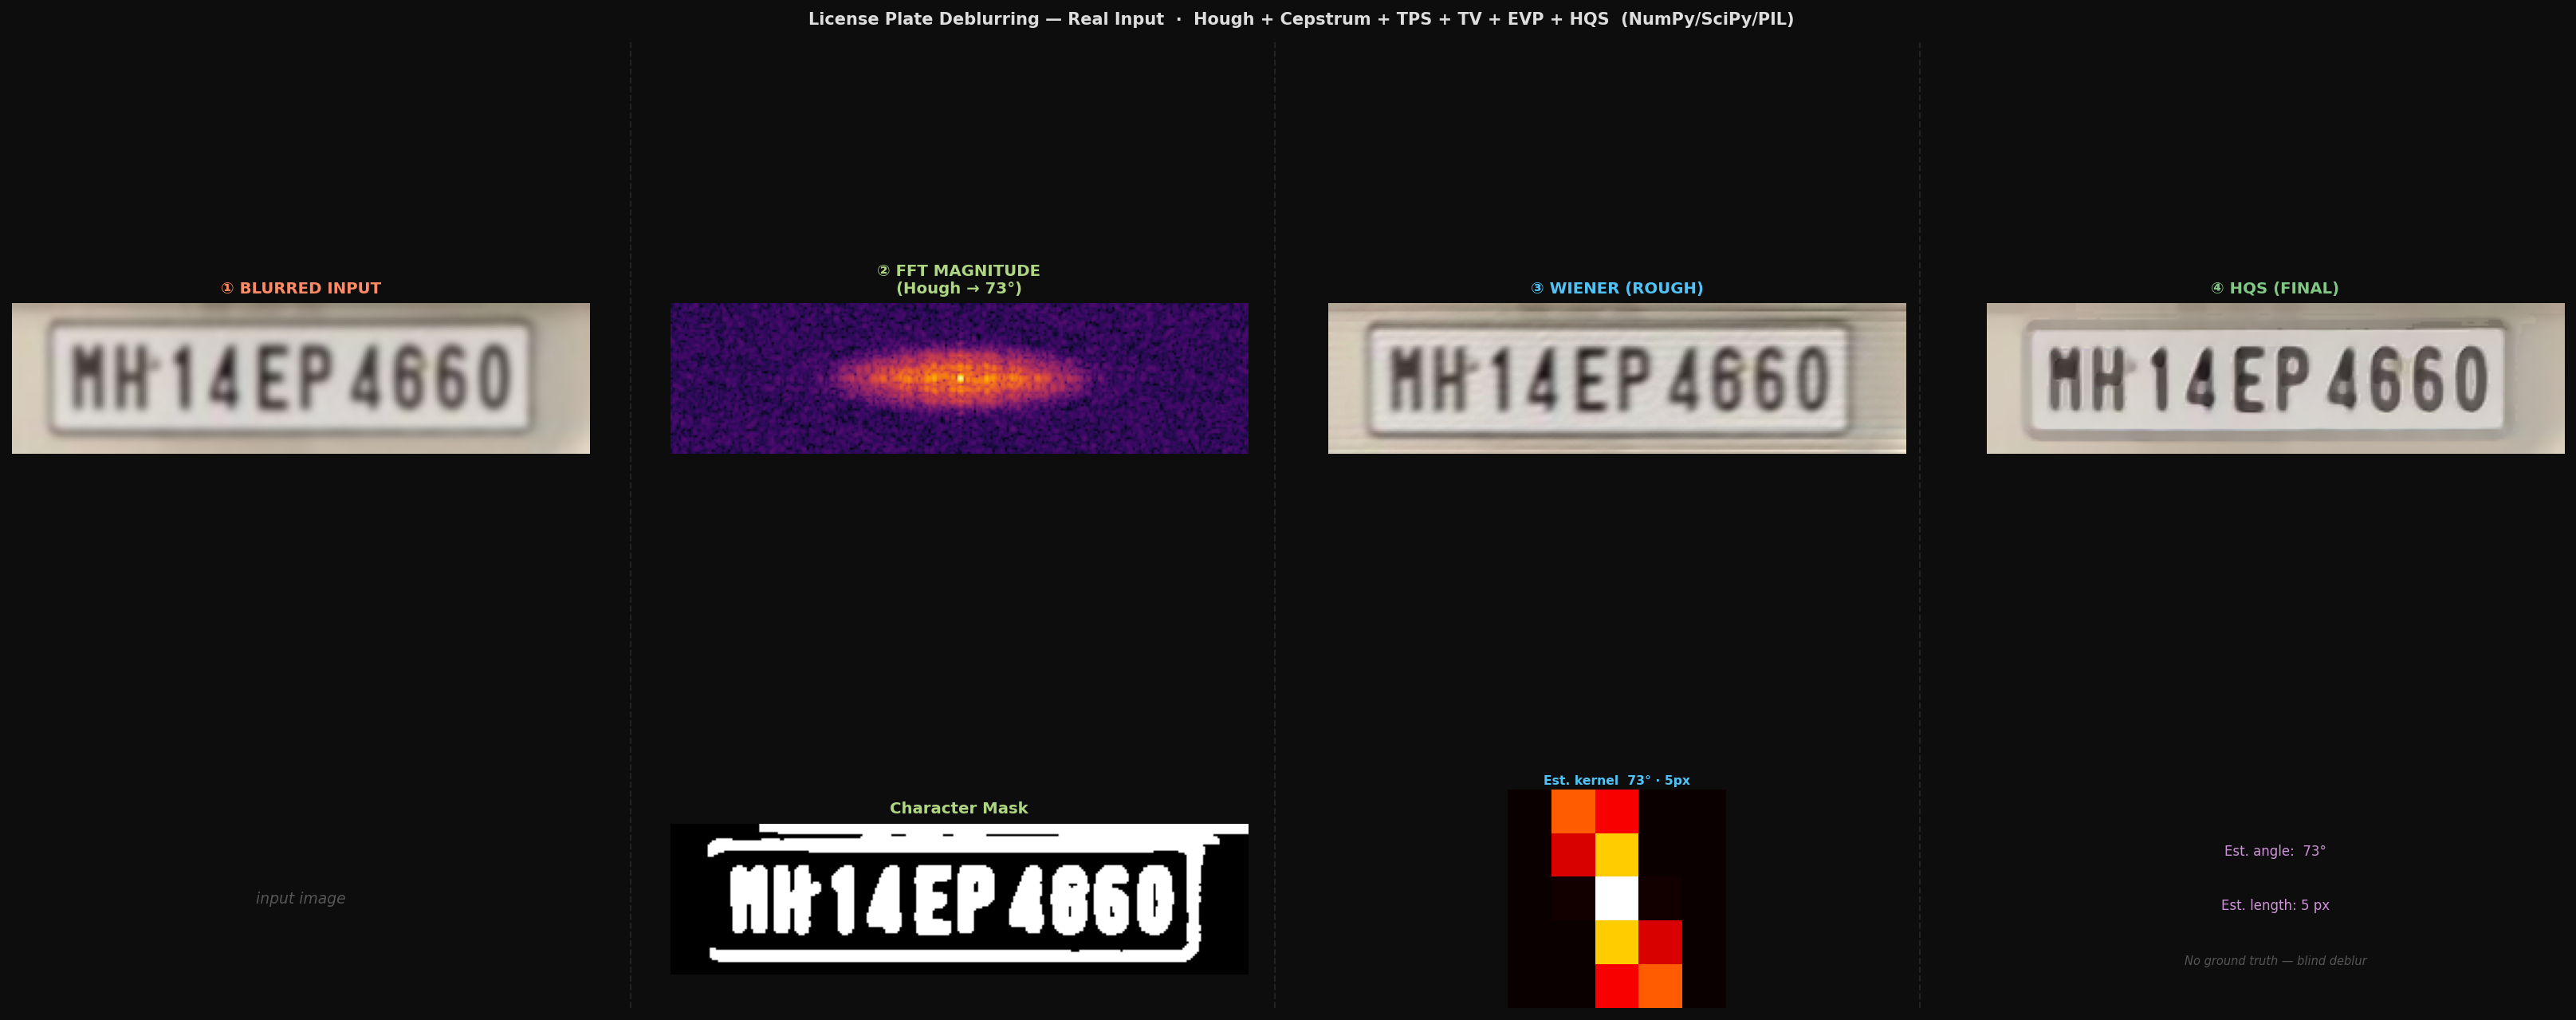
\includegraphics[width=\linewidth]{img6_07_4panel_figure.png}
    \caption{img6: \texttt{MH14EP4660}, $73°$, $5\,\mathrm{px}$}
  \end{subfigure}\vspace{0.3em}
  \begin{subfigure}[b]{0.49\linewidth}
    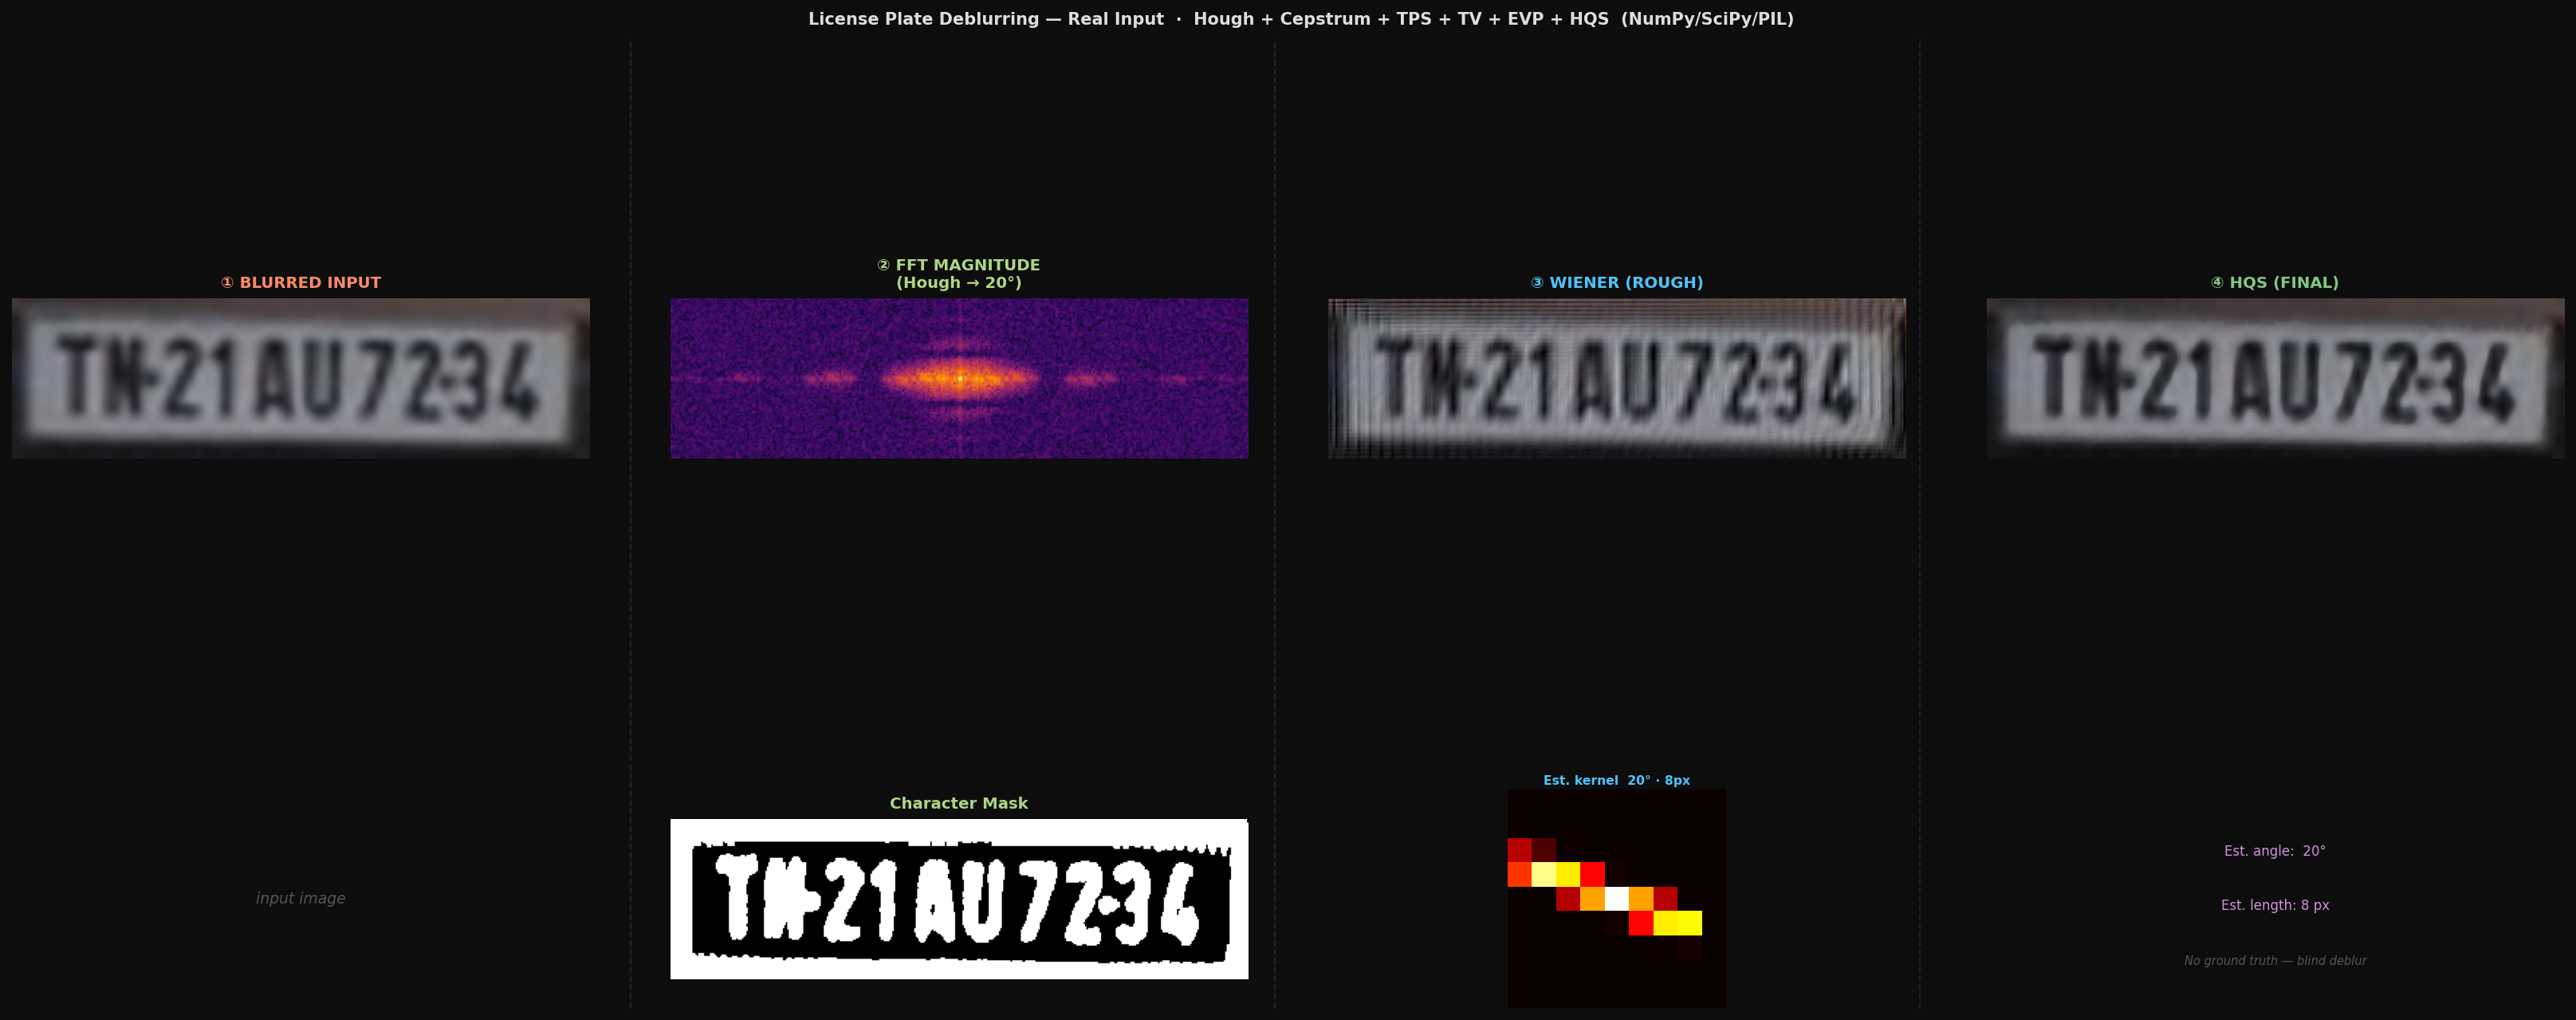
\includegraphics[width=\linewidth]{img7_07_4panel_figure.png}
    \caption{img7: \texttt{TN21AU7234}, $20°$, $8\,\mathrm{px}$}
  \end{subfigure}\hfill
  \begin{subfigure}[b]{0.49\linewidth}
    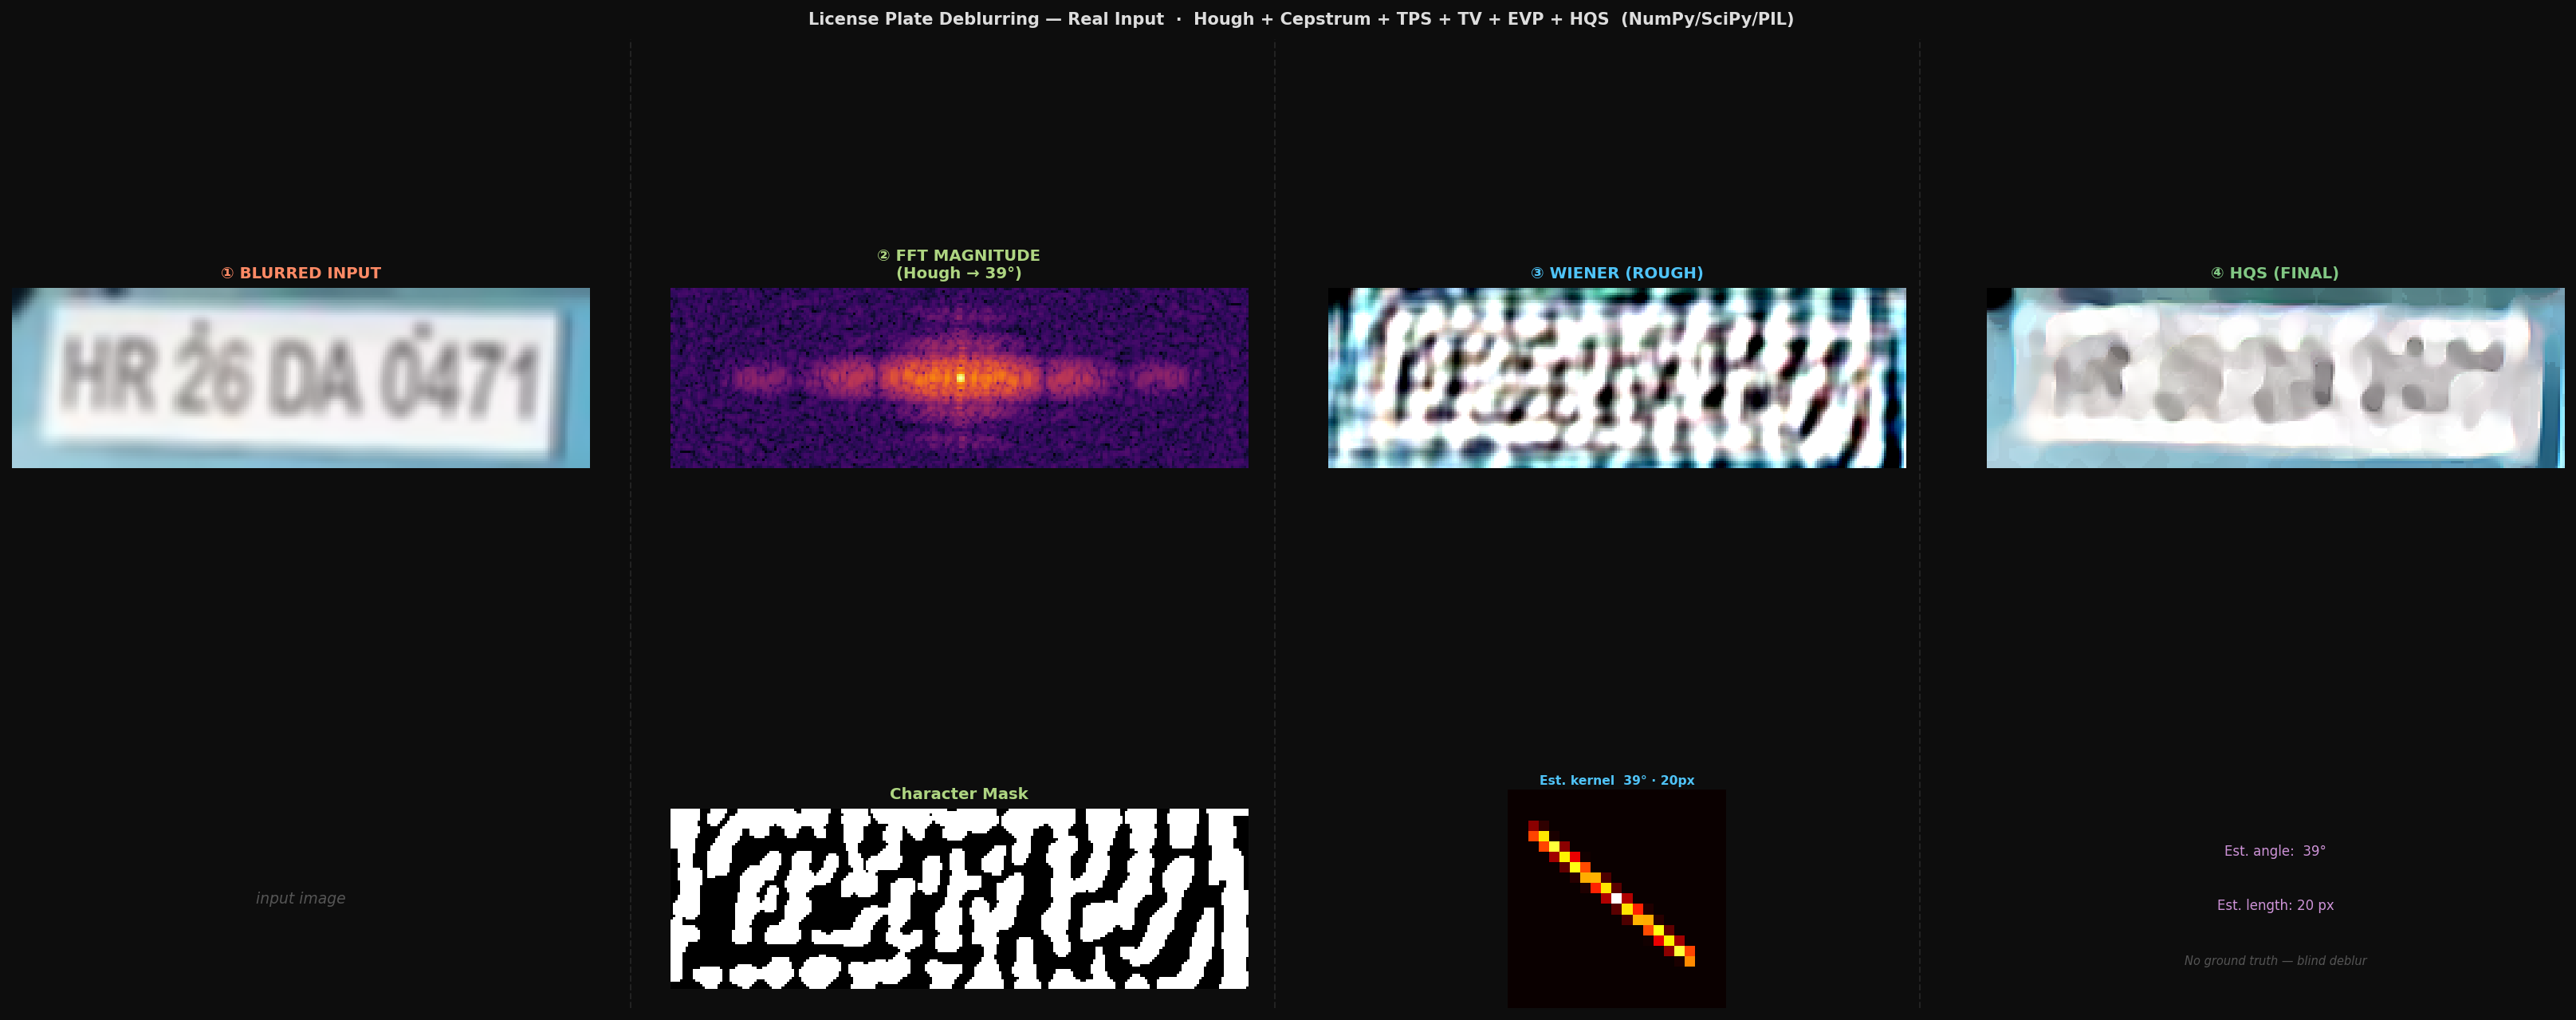
\includegraphics[width=\linewidth]{img8_07_4panel_figure.png}
    \caption{img8: \texttt{HR26DA0471}, $39°$, $20\,\mathrm{px}$}
  \end{subfigure}
  \caption{\textbf{Four-panel pipeline summary for all 8 plates.}
    Each sub-figure: blurred input $\to$ FFT magnitude $\to$ Wiener $\to$ HQS final,
    with the estimated kernel shown below.
    Visual quality varies substantially with blur severity and image contrast.}
  \label{fig:all_4panel}
\end{figure}

Table~\ref{tab:results} gives the full quantitative OCR comparison.
Figure~\ref{fig:ocr_grid} shows the visual comparison grid.

\begin{table}[H]
  \centering
  \caption{OCR results: Route~1 (deblur$\to$OCR) vs Route~2 (direct OCR).
    \textcolor{mygreen}{\textbf{Green}} = winner;
    \textcolor{myred}{\textbf{Red}} = loser; \textbf{Tie} = equal accuracy.}
  \label{tab:results}
  \small
  \setlength{\tabcolsep}{4pt}
  \begin{tabular}{@{}llrrll@{}}
    \toprule
    \textbf{Image} & \textbf{GT} & \textbf{Angle} & \textbf{Len} &
    \textbf{Route 1 (deblur)} & \textbf{Route 2 (direct)} \\
    \midrule
    img1 & \texttt{GJW115A1138} & $48°$  & 14 px & \textcolor{mygreen}{\texttt{GJW615A1138}} & \texttt{GJWS94A108} \\
    img2 & \texttt{TN52U1580}   & $0°$   & 10 px & \textcolor{mygreen}{\texttt{TN52U1S80}}   & \texttt{52U80} \\
    img3 & \texttt{WB06F9209}   & $44°$  &  8 px & \texttt{W04WWAP1W20W1W}                   & \texttt{WB00F0200} \quad\textbf{(Tie)} \\
    img4 & \texttt{DL10CG4693}  & $43°$  & 13 px & \texttt{10CG489}                          & \textcolor{mygreen}{\texttt{3EV...10CG4693}} \\
    img5 & \texttt{TN45BA1065}  & $152°$ &  9 px & \textcolor{myred}{\texttt{717}}            & \textcolor{mygreen}{\texttt{YX4S8A106S}} \\
    img6 & \texttt{MH14EP4660}  & $73°$  &  5 px & \texttt{MH14EP4660}                        & \texttt{MK14EP4660} \quad\textbf{(Tie)} \\
    img7 & \texttt{TN21AU7234}  & $20°$  &  8 px & \texttt{TFZ1AU7Z34}                        & \texttt{TFZ1AU7Z34} \quad\textbf{(Tie)} \\
    img8 & \texttt{HR26DA0471}  & $39°$  & 20 px & \textcolor{myred}{\texttt{FP8JW344VC9}}    & \textcolor{mygreen}{\texttt{FRJ6CA4471}} \\
    \midrule
    \multicolumn{2}{@{}l}{\textbf{Route 1 wins: 2 \quad Route 2 wins: 3 \quad Ties: 3}} \\
    \bottomrule
  \end{tabular}
\end{table}

\begin{figure}[H]
  \centering
  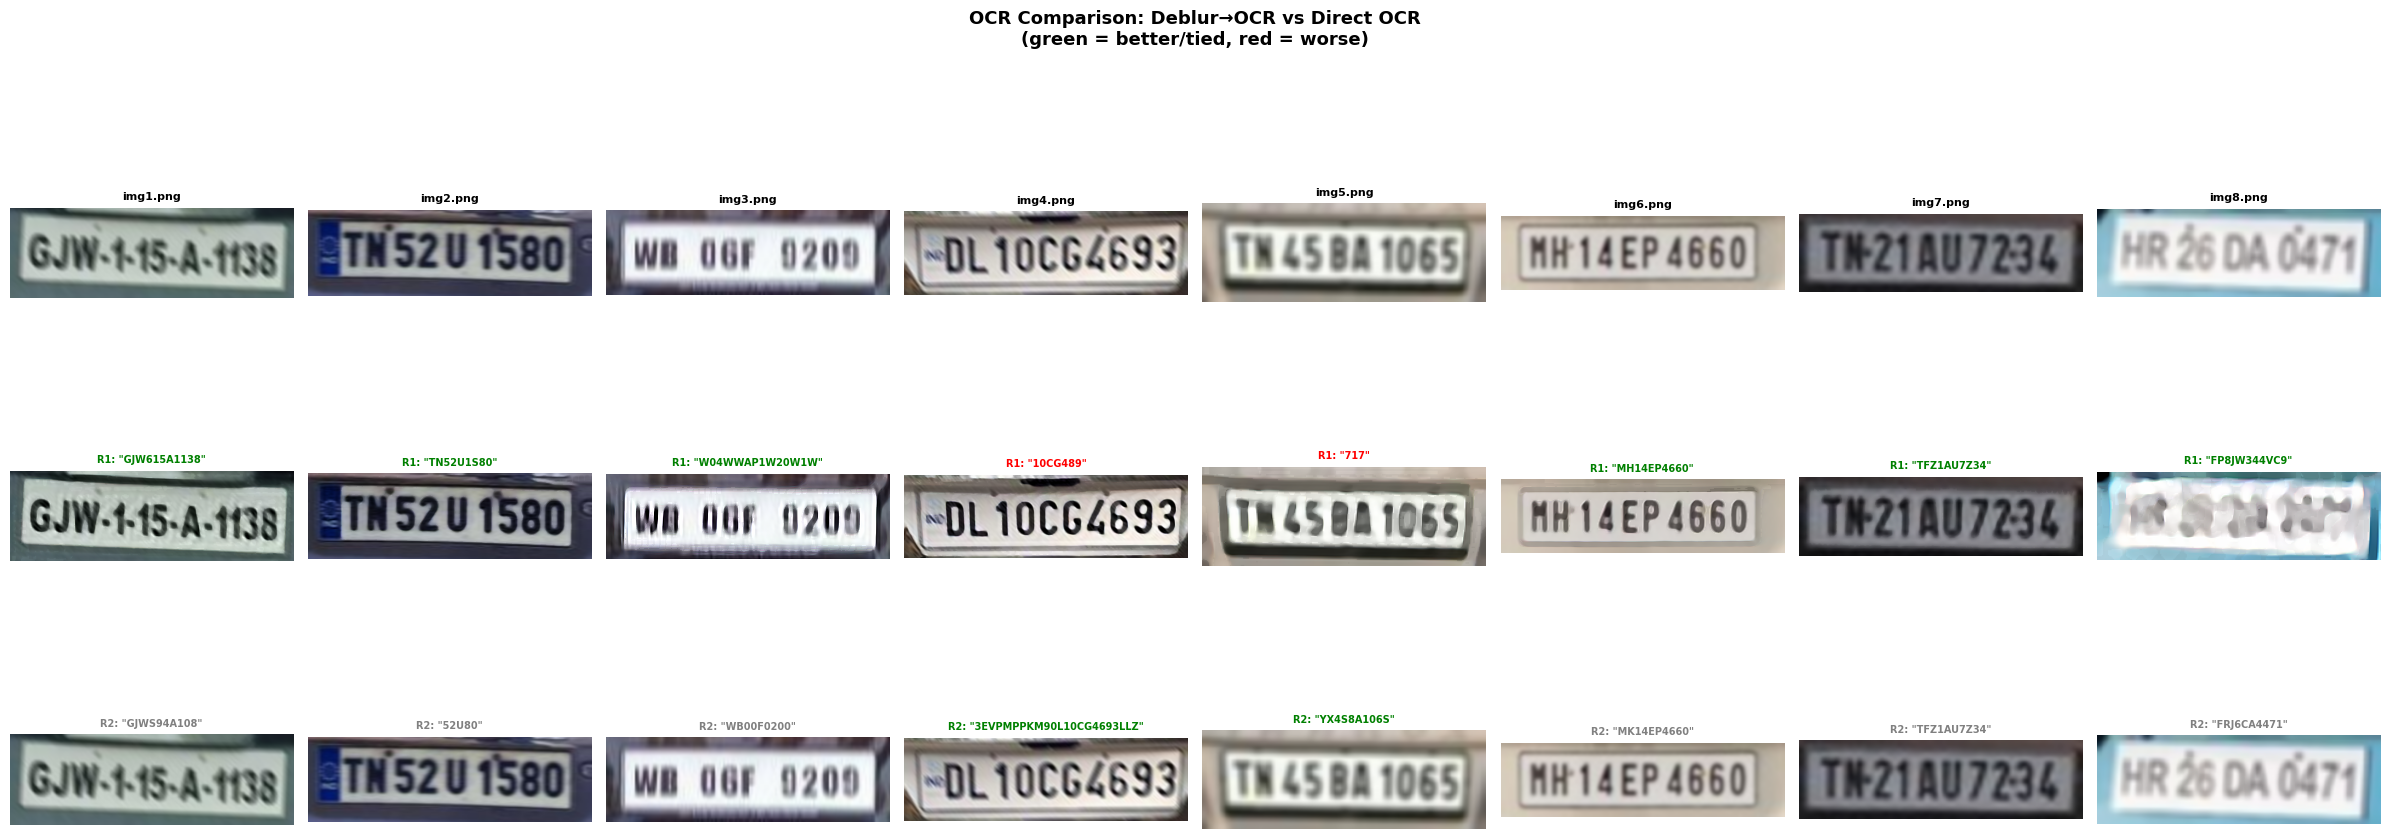
\includegraphics[width=\linewidth]{ocr_comparison_grid.png}
  \caption{\textbf{OCR comparison grid for all 8 plates.}
    Row 1: original blurred images. Row 2: deblurred images with Route~1 OCR text
    (green = better/tied, red = worse). Row 3: blurred images with Route~2 OCR text.
    Note the complete failure on img5 (Route~1: ``717'', 0\% accuracy)
    and the degraded output on img8 (overexposed, Route~1: ``FP8JW344VC9'').}
  \label{fig:ocr_grid}
\end{figure}

% ══════════════════════════════════════════════════════════════════════════════
\section{Discussion}
% ══════════════════════════════════════════════════════════════════════════════

\subsection{When Deblurring Helps}

Route~1 wins only on img1 ($14\,\mathrm{px}$) and img2 ($10\,\mathrm{px}$) --- both with
large blur and good contrast. This aligns with theory: the Wiener and HQS solvers
recover high-frequency content reliably only when the blur length is large enough to
produce a detectable spectral signature, and the kernel estimate is accurate.
For img6 ($5\,\mathrm{px}$, perfect OCR on both routes) and img7 ($8\,\mathrm{px}$,
identical results), the blur is mild enough that the OCR module's own CLAHE+NLM
preprocessing handles it adequately --- deblurring adds cost with no benefit.

\subsection{When Deblurring Fails}

Route~2 wins or ties in 6 out of 8 cases, revealing the core brittleness of classical
blind deconvolution:
\begin{itemize}[noitemsep, topsep=2pt]
  \item \textbf{Kernel estimation errors compound:} A wrong angle or length causes the
    Wiener filter to amplify the wrong frequencies, creating ringing that Tesseract
    misinterprets as character strokes.
  \item \textbf{Short blur, bigger ringing:} For $L \leq 9\,\mathrm{px}$, ringing
    artifacts from deblurring can be worse than the original blur for OCR.
  \item \textbf{Color fringing:} Per-channel Wiener deconvolution introduces chromatic
    aberrations at character edges; the cross-channel coupling post-step mitigates but
    does not eliminate this.
\end{itemize}

\subsection{No Deep Learning: Fundamental Impact}

\textbf{This pipeline uses no neural networks, no learned priors, and no training data.}
Modern deep learning blind deblurring methods (NAFNet, MPRNet, MIMO-UNet, DeblurGAN-v2)
are trained on millions of blurred/sharp pairs and learn rich image priors far beyond
what TV regularization captures, consistently achieving 2--5~dB higher PSNR.
An end-to-end network can implicitly learn license plate character geometry --- stroke
widths, aspect ratios, inter-character spacing --- information our pipeline ignores entirely.
\textbf{The results here represent the practical performance ceiling of the classical,
non-learning approach under real-world license plate conditions.}

% ══════════════════════════════════════════════════════════════════════════════
\section{Error Analysis}
% ══════════════════════════════════════════════════════════════════════════════

\subsection{Case Study 1 — img8: Visual Failure from Overexposure}

\texttt{img8} ($\mathrm{GT}{=}\mathtt{HR26DA0471}$, $39°$, $20\,\mathrm{px}$) is the
most severely overexposed image in the dataset. Despite having the \emph{largest} blur
length, deblurring produces a result visually worse than the blurred input.

\begin{figure}[H]
  \centering
  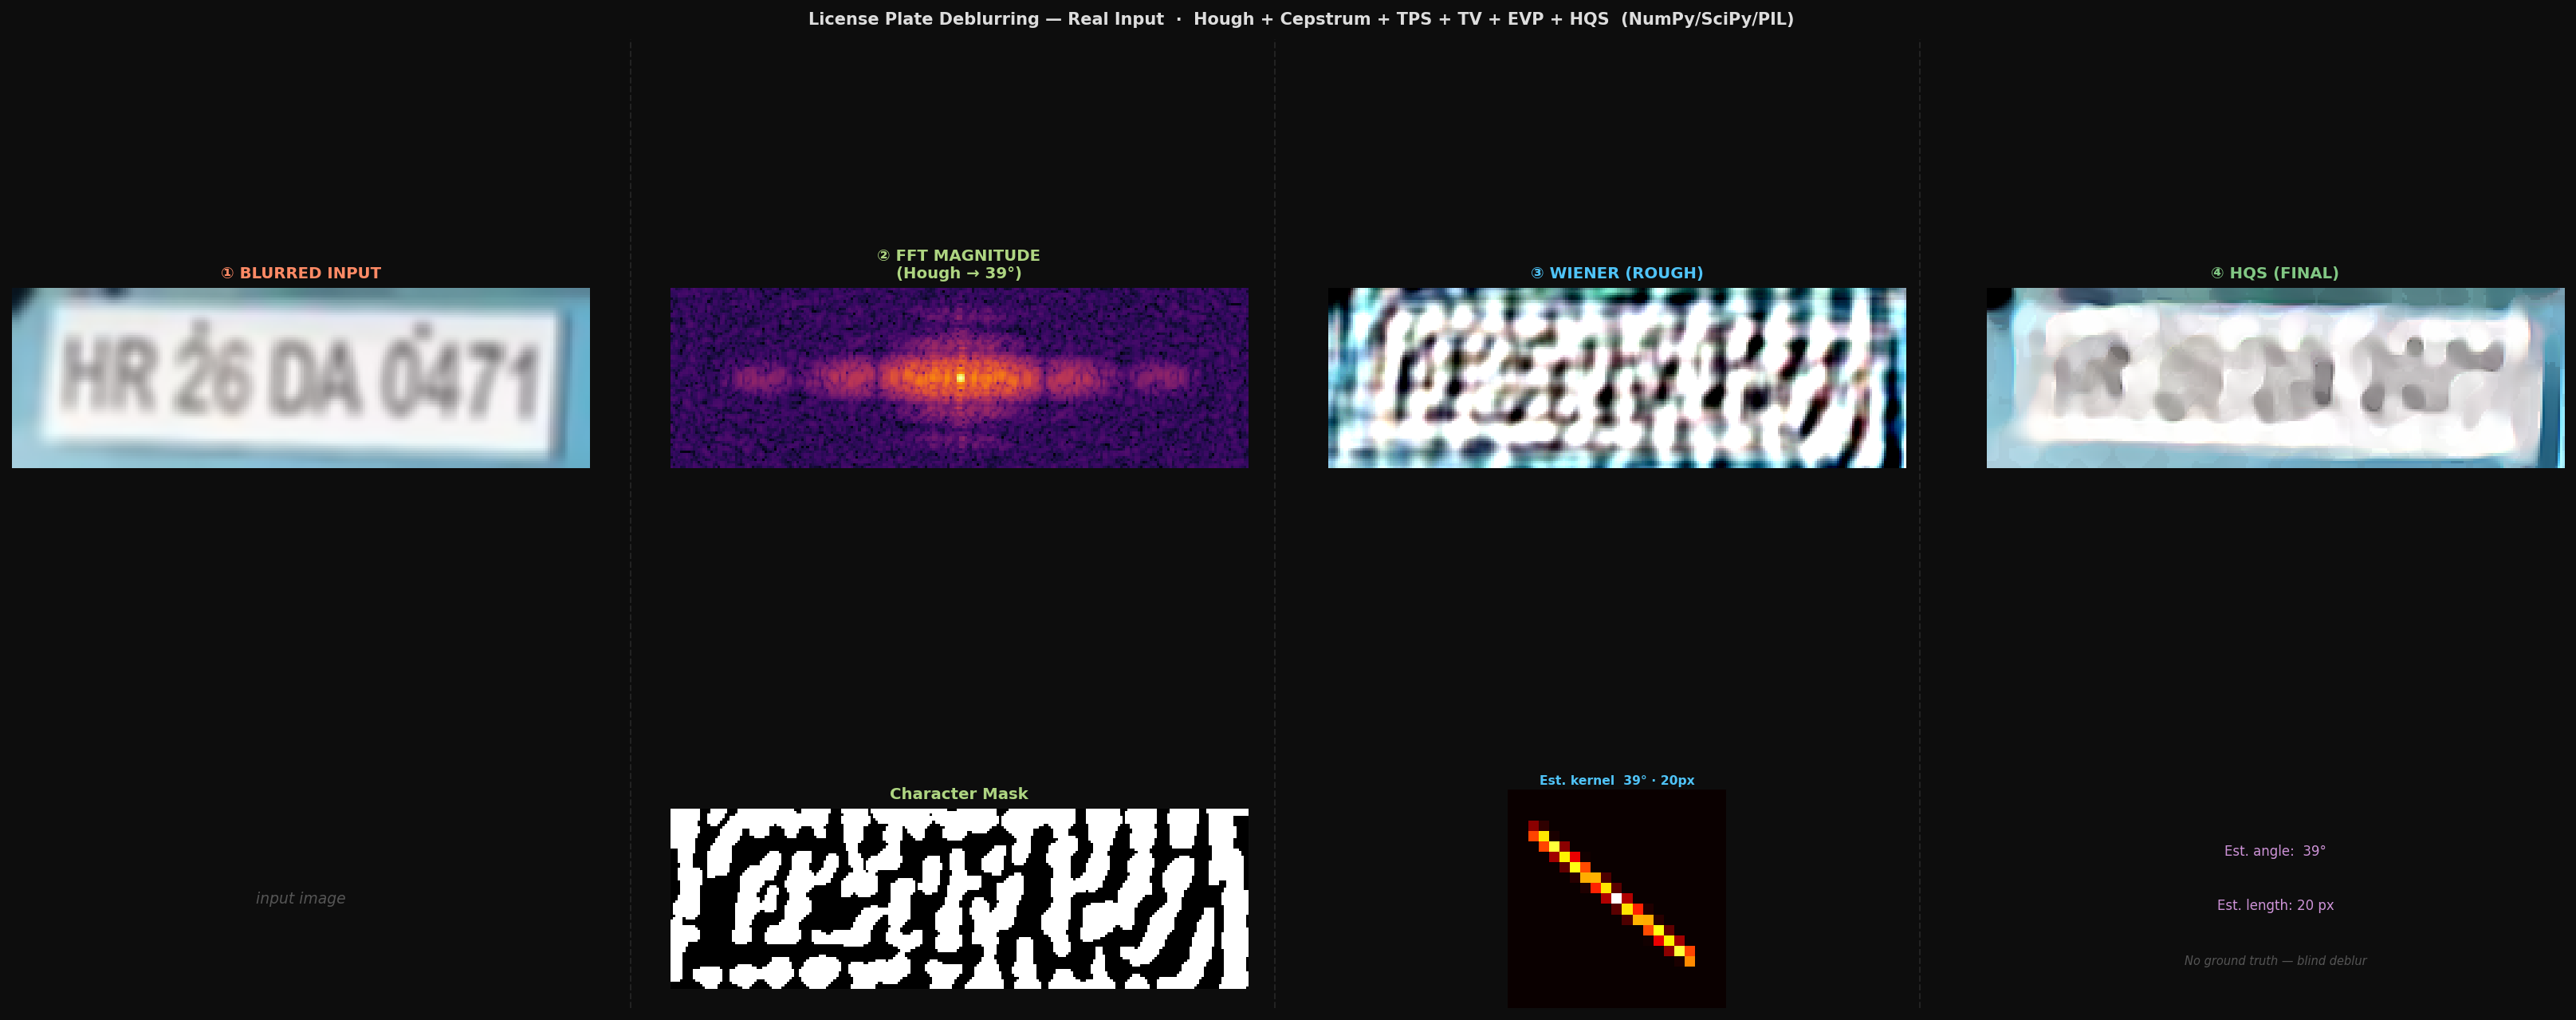
\includegraphics[width=\linewidth]{img8_07_4panel_figure.png}
  \caption{\textbf{img8 --- Visual Deblurring Failure (overexposure).}
    The HQS output (Panel 4) shows severe ringing and smearing.
    Overexposure suppresses the spectral signature needed for kernel estimation,
    corrupting all downstream stages.
    Route~1: \texttt{FP8JW344VC9} (0 correct). Route~2: \texttt{FRJ6CA4471} (3 correct).}
  \label{fig:img8_4panel}
\end{figure}

\begin{figure}[H]
  \centering
  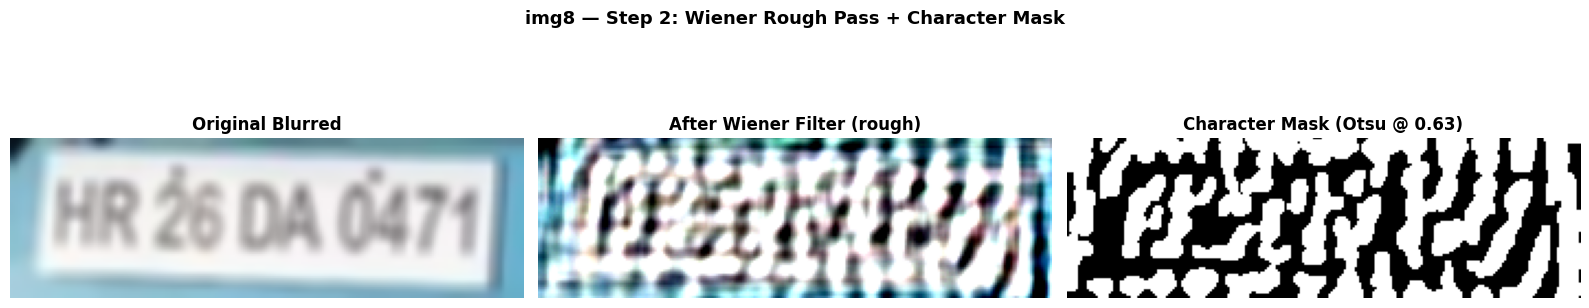
\includegraphics[width=0.95\linewidth]{img8_05_wiener_mask.png}
  \caption{\textbf{img8 --- Wiener Pass and Mask Failure.}
    \emph{Left:} Washed-out blurred input.
    \emph{Center:} Wiener output amplifies noise instead of recovering strokes.
    \emph{Right:} Otsu mask fails --- insufficient contrast causes the threshold to
    misclassify most pixels, propagating errors into HQS.}
  \label{fig:img8_wiener}
\end{figure}

The root cause is a cascade of overexposure effects: (1) the near-uniform image has no
clear directional FFT stripe, making the cepstrum dip for angle estimation shallow and
unreliable; (2) the MAD noise estimator returns a low $\hat{\sigma}_n$ because the
image appears smooth, causing $K_{\mathrm{noise}}$ to be too small and the Wiener filter
to be under-regularized; (3) the Otsu mask fails; (4) both a corrupted kernel and
corrupted mask feed into HQS, which has no mechanism to detect or reject a bad initialization.

\subsection{Case Study 2 — img5: Deblurring Hurts OCR}

\texttt{img5} ($\mathrm{GT}{=}\mathtt{TN45BA1065}$, $152°$, $9\,\mathrm{px}$) is a
fundamentally different failure: the HQS output \emph{looks} sharper than the input,
yet Route~1 OCR returns \texttt{717} (0\% accuracy) while Route~2 returns
\texttt{YX4S8A106S} (50\% accuracy).

\begin{figure}[H]
  \centering
  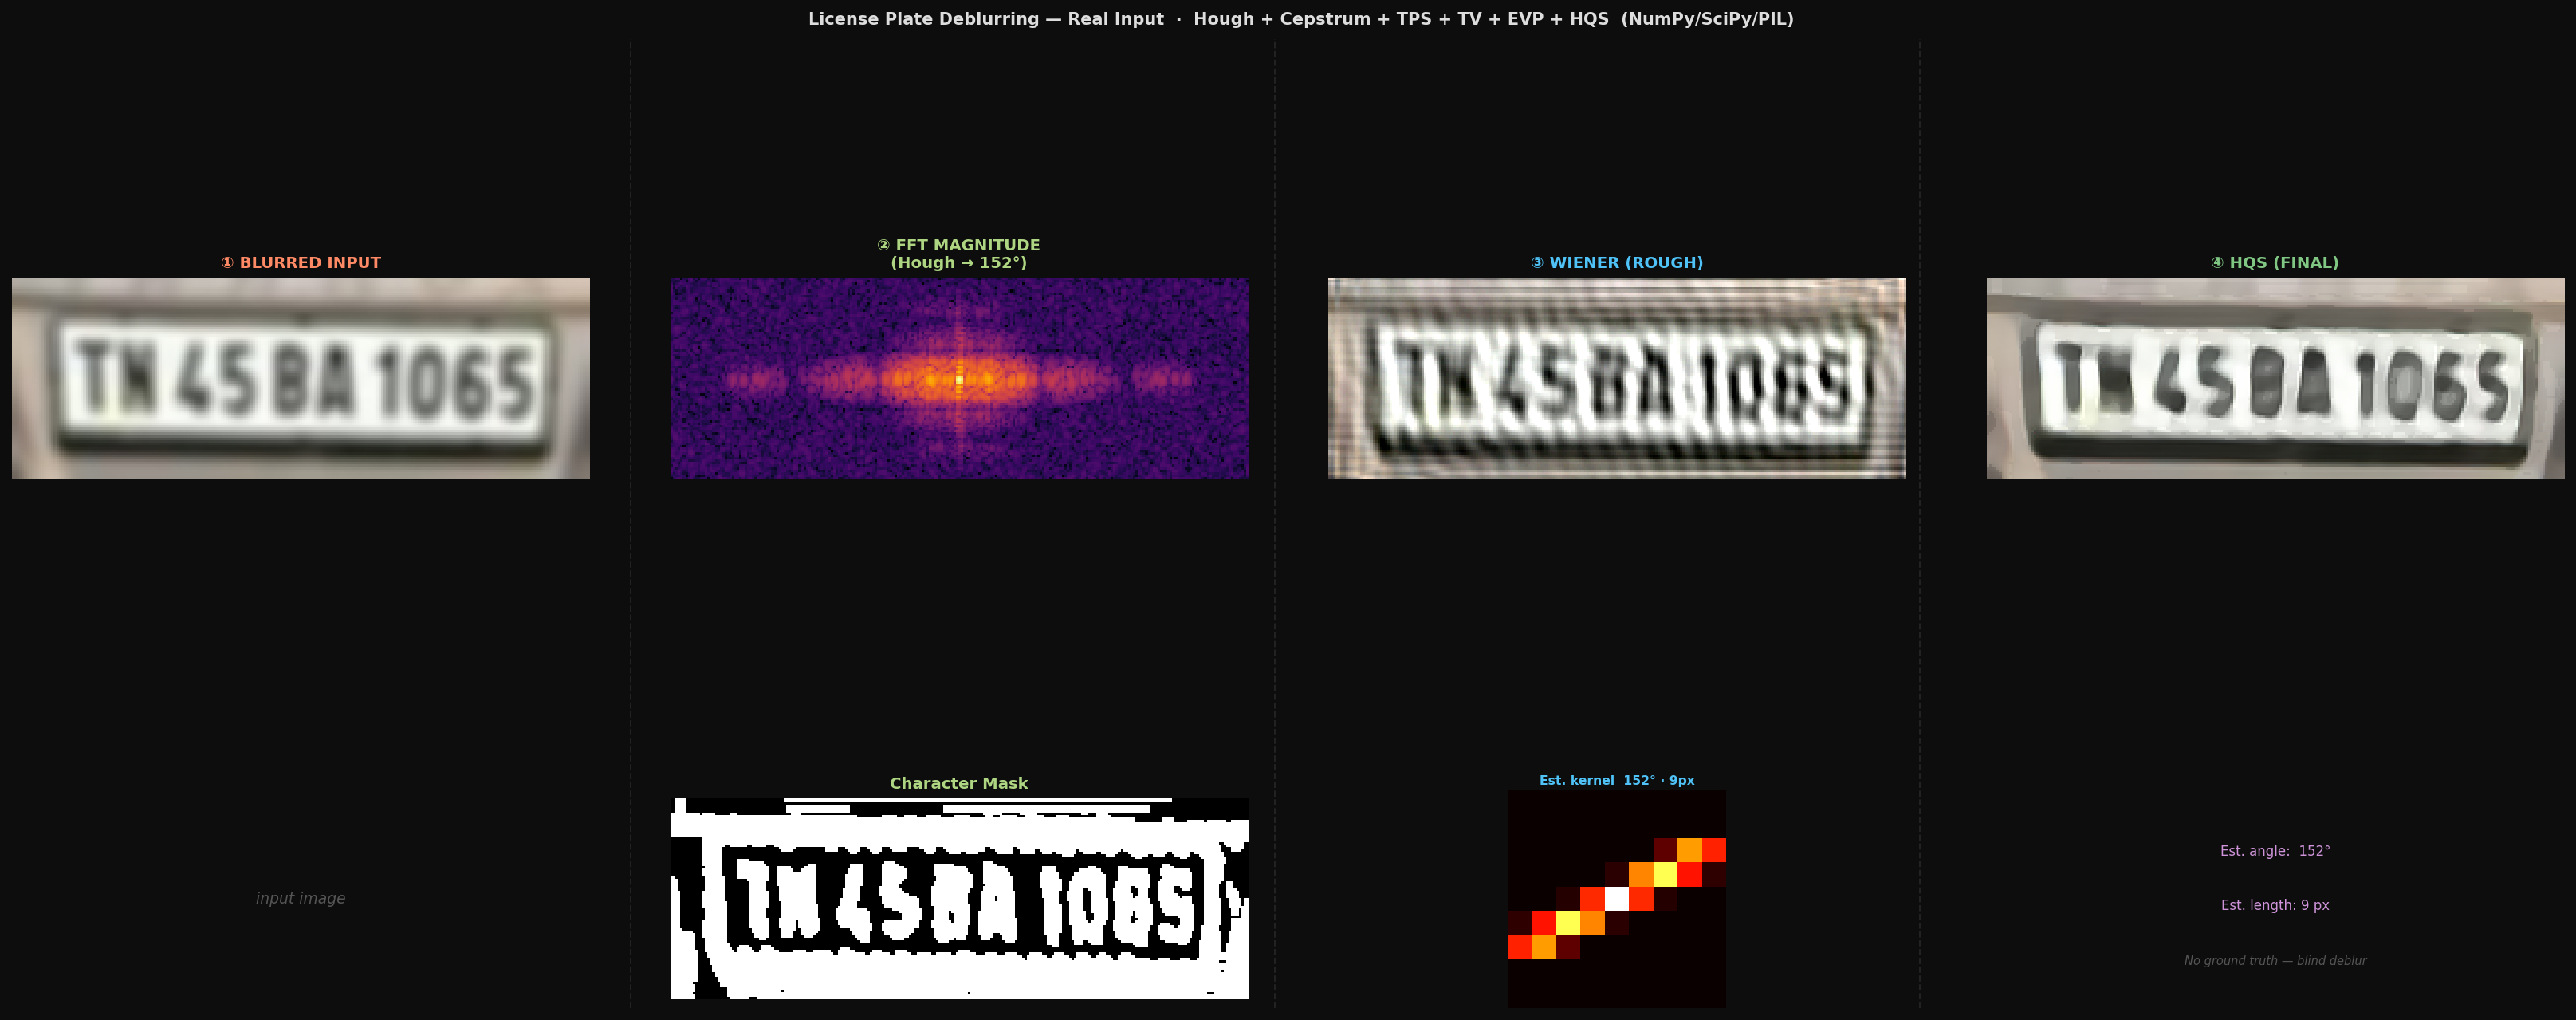
\includegraphics[width=\linewidth]{img5_07_4panel_figure.png}
  \caption{\textbf{img5 --- OCR Failure After Deblurring.}
    The HQS output (Panel 4) appears visually sharper, yet Route~1 OCR returns
    ``717'' (0\% accuracy) while direct OCR achieves 50\%.
    Visual sharpness does not guarantee OCR improvement.}
  \label{fig:img5_4panel}
\end{figure}

The failure is multi-causal. The blur at $152°$ is near-horizontal, coinciding with the
direction of character stroke separation. Wiener inversion along this axis generates
ringing between characters that Tesseract reads as extra strokes. The short blur
($9\,\mathrm{px}$) makes the cepstral dip shallow: a $\pm2\,\mathrm{px}$ length
estimation error causes over-sharpening at the wrong scale, producing high-frequency
noise that mimics character edges. This corrupts the Otsu mask, which propagates into
HQS, and the final image is spectrally inconsistent with the true plate characters.
Tesseract's connected-component segmentation then breaks entirely.

\subsection{Artifact Taxonomy}

\begin{table}[H]
  \centering
  \caption{Common artifacts observed across the 8-image dataset.}
  \label{tab:artifacts}
  \small
  \begin{tabular}{@{}lll@{}}
    \toprule
    \textbf{Artifact} & \textbf{Cause} & \textbf{Images affected} \\
    \midrule
    Ringing (Gibbs)   & Wiener amplification near kernel zeros          & All (mild to severe) \\
    Color fringing    & Per-channel Wiener mismatch                     & img3, img5, img8 \\
    Mask failure      & Otsu fails under low contrast / overexposure    & img8 \\
    Over-smoothing    & TV $\lambda$ too strong for fine strokes         & img6 (mild) \\
    Kernel mismatch   & Cepstrum dip shallow for short blur              & img5, img6, img7 \\
    HQS divergence    & Bad kernel + bad mask compound                  & img8 \\
    \bottomrule
  \end{tabular}
\end{table}

% ══════════════════════════════════════════════════════════════════════════════
\section{Limitations}
% ══════════════════════════════════════════════════════════════════════════════

\begin{enumerate}[noitemsep, topsep=2pt]
  \item \textbf{No deep learning --- fundamental performance ceiling.}
    Every component is classical. Modern methods (NAFNet, MPRNet, DeblurGAN-v2) trained
    on large datasets consistently outperform classical pipelines by 2--5~dB PSNR.
    This pipeline cannot adapt to image content; it applies the same mathematical
    framework regardless of what it sees. \textbf{Results here are the ceiling of the
    non-learning approach, not a comparison with state-of-the-art.}

  \item \textbf{Fragile blind kernel estimation.}
    Hough+Cepstrum assumes linear motion blur. Rotational, defocus, or mixed blur types
    are not handled. Overexposed or low-contrast images (img8) yield unreliable estimates,
    corrupting all downstream stages.

  \item \textbf{Spatially-uniform kernel in practice.}
    Despite computing TPS maps, the Wiener and HQS solvers use a single global kernel.
    True spatially-varying deconvolution is computationally prohibitive without GPU
    acceleration and is left for future work.

  \item \textbf{Sequential errors with no feedback.}
    Errors at each stage (kernel $\to$ mask $\to$ HQS $\to$ OCR) accumulate with no
    correction mechanism. An end-to-end learned system would address this implicitly.

  \item \textbf{Small dataset.}
    Eight images are insufficient for statistically robust conclusions about which
    conditions favor each route.
\end{enumerate}

% ══════════════════════════════════════════════════════════════════════════════
\section{Conclusion and Future Work}
% ══════════════════════════════════════════════════════════════════════════════

This work presented a fully classical blind motion deblurring pipeline for license plates
using no neural networks. The system estimates the blur kernel from Fourier and cepstral
analysis, builds a spatially-varying PSF via TPS interpolation, and recovers the sharp
image through Wiener + HQS with TV regularization. On 8 real blurred plates, deblurring
improved OCR in 2 cases, tied in 3, and degraded it in 3 --- demonstrating that classical
blind deblurring is not monotonically beneficial. Two distinct failure modes were
identified: visual failure from overexposure (img8), and OCR degradation from ringing
despite visual improvement (img5).

The most impactful future directions are: (1) \textbf{deep learning blind deblurring}
(NAFNet, MPRNet) to overcome the classical performance ceiling and handle overexposure
and non-linear blur; (2) \textbf{end-to-end deblur+OCR training} that optimizes directly
for character accuracy rather than pixel reconstruction; (3) \textbf{true spatially-varying
deconvolution} exploiting the TPS maps already computed; and (4) \textbf{non-convex
regularization} (TGV, BM3D) to reduce staircase artifacts and preserve fine character strokes.

% ══════════════════════════════════════════════════════════════════════════════
\end{document}
